\chapter{Managing a Hadoop Cluster}\label{chap:4}
In this chapter, we will cover: \\
\begin{itemize}
  \item Managing HDFS cluster
  \item Configuring SecondaryNameNode
  \item Managing MapReduce cluster
  \item Managing TaskTracker
  \item Decommissioning DataNode
  \item Replacing a slave node
  \item Managing MapReduce jobs
  \item Checking job history from the web UI
  \item Importing data to HDFS
  \item Manipulating files on HDFS
  \item Configuring HDFS quota
  \item Configuring CapacityScheduler
  \item Configuring fair scheduler
  \item Configuring Hadoop daemon logging
  \item Configuring Hadoop audit logging
  \item Upgrading Hadoop
\end{itemize}

\section{Introduction}
From the perspective of functionality, a Hadoop cluster is composed of an HDFS cluster and a MapReduce cluster. The HDFS cluster consists of the default filesystem for Hadoop. It has one or more NameNodes to keep track of the filesystem metadata, while actual data blocks are stored on distributed slave nodes managed by DataNode. Similarly, a MapReduce cluster has one JobTracker on the master node and a number of TaskTrackers on the slave nodes. The JobTracker manages the life cycle of MapReduce jobs. It splits jobs into smaller tasks and schedules the tasks to run by the TaskTrackers. A TaskTracker executes tasks assigned by the JobTracker in parallel by forking one or a number of JVM processes. As a Hadoop cluster administrator, you will be responsible for managing both the HDFS cluster and the MapReduce cluster.

In general, system administrators should maintain the health and availability of the cluster. More specifically, for a HDFS cluster, it means the management of the NameNodes and DataNodes and the management of the JobTrackers and TaskTrackers for MapReduce. Other administrative tasks include the management of Hadoop jobs, for example configuring job scheduling policy with schedulers.

At the end of this chapter, we will cover topics for configuring Hadoop logging and doing system upgrade. Logging provides insights for diagnosing cluster failure or performance problems, and system upgrade plays an important role in keeping the software up to date.

\subsection*{Managing HDFS cluster}
The health of HDFS\index{HDFS} is critical for a Hadoop-based Big Data platform. HDFS problems can negatively affect the efficiency of the cluster. Even worse, it can make the cluster not function properly. For example, DataNode unavailability caused by network segmentation\index{network segmentation} can lead to some under-replicated data blocks. When this happens, HDFS will automatically replicate those data blocks, which will bring a lot of overhead to the cluster and cause the cluster to be too unstable to be available for use. In this recipe, we will show commands to manage a HDFS cluster.
\subsection*{Getting ready}
Before getting started, we assume that our Hadoop cluster has been properly configured and all the daemons are running without any problems.
Log in to the master node from the administrator machine with the following command:
ssh hduser@master
\subsection*{How to do it...}
Use the following steps to check the status of a HDFS cluster with \verb|hadoop fsck|\index{hadoop fsck}:

Check the status of the root filesystem\index{root filesystem} with the following command:
\lstset{style=bashstyle}
\begin{lstlisting}
$ hadoop fsck /
FSCK started by hduser from /10.147.166.55 for path / at Thu Feb 28 17:14:11 EST 2013
..
/user/hduser/.staging/job_201302281211_0002/job.jar:  Under replicated blk_-665238265064328579_1016. Target Replicas is 10 but found 5 replica(s).
.................................Status: HEALTHY
 Total size:    14420321969 B
 Total dirs:    22
 Total files:   35
 Total blocks (validated):      241 (avg. block size 59835360 B)
 Minimally replicated blocks:   241 (100.0 %)
 Over-replicated blocks:        0 (0.0 %)
 Under-replicated blocks:       2 (0.8298755 %)
 Mis-replicated blocks:         0 (0.0 %)
 Default replication factor:    2
 Average block replication:     2.0248964
 Corrupt blocks:                0
 Missing replicas:              10 (2.0491803 %)
 Number of data-nodes:          5
 Number of racks:               1
FSCK ended at Thu Feb 28 17:14:11 EST 2013 in 28 milliseconds

The filesystem under path '/' is HEALTHY
\end{lstlisting}

The output shows that some percentage of data blocks is under replicated\index{under replicated}. But because HDFS can automatically make duplication for those data blocks, the HDFS filesystem and the '/' directory are both HEALTHY.

Check the status of all the files on HDFS with the following command:
\lstset{style=bashstyle}
\begin{lstlisting}
$ hadoop fsck / -files
FSCK started by hduser from /10.147.166.55 for path / at Thu Feb 28 17:40:35 EST 2013
/ <dir>
/home <dir>
/home/hduser <dir>
/home/hduser/hadoop <dir>
/home/hduser/hadoop/tmp <dir>
/home/hduser/hadoop/tmp/mapred <dir>
/home/hduser/hadoop/tmp/mapred/system <dir>
/home/hduser/hadoop/tmp/mapred/system/jobtracker.info 4 bytes, 1 block(s):  OK
/user <dir>
/user/hduser <dir>
/user/hduser/randtext <dir>
/user/hduser/randtext/_SUCCESS 0 bytes, 0 block(s):  OK
/user/hduser/randtext/_logs <dir>
/user/hduser/randtext/_logs/history <dir>
/user/hduser/randtext/_logs/history/job_201302281451_0002_1362090421087_hduser_random-text-writer 23995 bytes, 1 block(s):  OK
/user/hduser/randtext/_logs/history/job_201302281451_0002_conf.xml 22878 bytes, 1 block(s):  OK
/user/hduser/randtext/part-00001 1102231864 bytes, 17 block(s):  OK
Status: HEALTHY
\end{lstlisting}
Hadoop will scan and list all the files in the cluster.

This command scans all files on HDFS and prints the size and status.

Check the locations of file blocks\index{file blocks} with the following command: \\
\verb|$ hadoop fsck / -files -locations|

The output will be similar to Figure \ref{fig:hdfs.block.locations}.
\begin{figure}[ht]
  \centering
  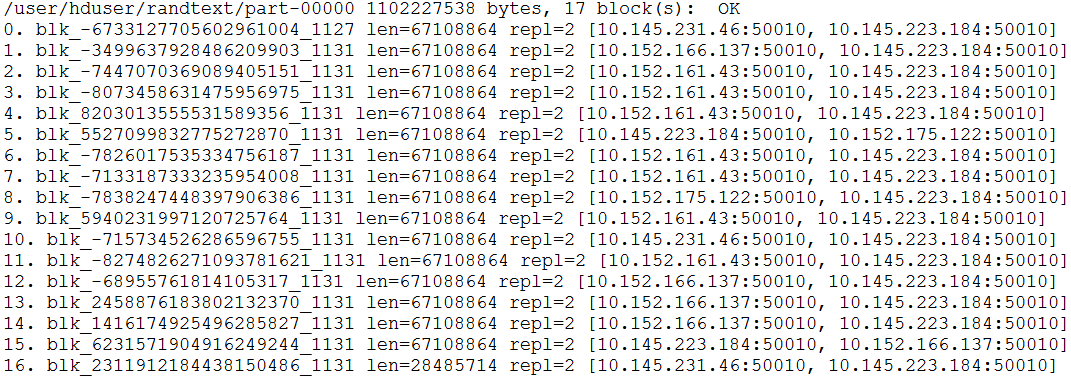
\includegraphics[width=.95\textwidth]{figs/5163os_04_07.png}
  \caption{Block locations on HDFS}\label{fig:hdfs.block.locations}
\end{figure} 
The first line tells us that file \verb|part-00000| has 17 blocks in total and each block has 2 replications (replication factor\index{replication factor} has been set to 2). The following lines list the location of each block on the DataNode. For example, block \verb|blk_6733127705602961004_1127| has been replicated on hosts \verb|10.145.231.46| and \verb|10.145.223.184|. The number 50010 is the port number of the DataNode\index{DataNode port number}.

Check the locations of file blocks containing rack\index{rack} information with the following command: \\
\verb|$ hadoop fsck / -files -blocks -racks|

Delete corrupted files\index{corrupted files} with the following command:\\
\verb|$ hadoop fsck -delete|

Move corrupted files to /lost+found\index{lost+found} with the following command: \\
\verb|$ hadoop fsck -move|

Use the following steps to check the status of a HDFS cluster with hadoop dfsadmin:

Report the status of each slave node with the following command: 
\lstset{style=bashstyle}
\begin{lstlisting}
$ hadoop dfsadmin -report
Configured Capacity: 422797230080 (393.76 GB)
Present Capacity: 399233617920 (371.82 GB)
DFS Remaining: 388122796032 (361.47 GB)
DFS Used: 11110821888 (10.35 GB)
DFS Used%: 2.78%
Under replicated blocks: 0
Blocks with corrupt replicas: 0
Missing blocks: 0

-------------------------------------------------
Datanodes available: 5 (5 total, 0 dead)

Name: 10.145.223.184:50010
Decommission Status : Normal
Configured Capacity: 84559446016 (78.75 GB)
DFS Used: 2328719360 (2.17 GB)
Non DFS Used: 4728565760 (4.4 GB)
DFS Remaining: 77502160896(72.18 GB)
DFS Used%: 2.75%
DFS Remaining%: 91.65%
Last contact: Thu Feb 28 20:30:11 EST 2013

...

\end{lstlisting}

The first section of the output shows the summary of the HDFS cluster, including the configured capacity\index{capacity}, present capacity\index{present capacity}, remaining capacity\index{remaining capacity}, used space, number of under replicated data blocks, number of data blocks with corrupted replicas\index{corrupted replicas}, and number of missing blocks\index{missing blocks}.

The following sections of the output information show the status of each HDFS slave node, including the name (ip:port) of DataNode machine, commission status, configured capacity, HDFS and non-HDFS used space amount, HDFS remaining space, and the time that the slave node contacted the master.

Refresh all the DataNodes using the following command: \\
\verb|$ hadoop dfsadmin -refreshNodes|

Check the status of the safe mode\index{safe mode} using the following command:
\lstset{style=bashstyle}
\begin{lstlisting}
$ hadoop dfsadmin -safemode get
Safe mode is OFF
\end{lstlisting}

The output tells us that the NameNode is not in safe mode. In this case, the filesystem is both readable and writable. If the NameNode is in safe mode, the filesystem will be read-only (write protected).

Manually put the NameNode into safe mode using the following command: \\
\verb|$ hadoop dfsadmin -safemode enter|

This command is useful for system maintenance.

Make the NameNode to leave safe mode using the following command: \\
\verb|$ hadoop dfsadmin -safemode leave|

If the NameNode has been in safe mode for a long time or it has been put into safe mode manually, we need to use this command to let the NameNode leave this mode.

Wait until NameNode leaves safe mode using the following command:\\
\verb|$ hadoop dfsadmin -safemode wait|\\
This command is useful when we want to wait until HDFS finishes data block replication or wait until a newly commissioned DataNode\index{newly commissioned DataNode} to be ready for service.

Save the metadata of the HDFS\index{HDFS metadata} filesystem with the following command: \\
\verb|$ hadoop dfsadmin -metasave meta.log|

The meta.log file will be created under the directory \verb|$HADOOP_HOME/logs|. Its content will be similar to the following:
\lstset{style=bashstyle}
\begin{lstlisting}
21 files and directories, 88 blocks = 109 total
Live Datanodes: 5
Dead Datanodes: 0
Metasave: Blocks waiting for replication: 0
Metasave: Blocks being replicated: 0
Metasave: Blocks 0 waiting deletion from 0 datanodes.
Metasave: Number of datanodes: 5
10.145.223.184:50010 IN 84559446016(78.75 GB) 2328719360(2.17 GB) 2.75% 77502132224(72.18 GB) Thu Feb 28 21:43:52 EST 2013
10.152.166.137:50010 IN 84559446016(78.75 GB) 2357415936(2.2 GB) 2.79% 77492854784(72.17 GB) Thu Feb 28 21:43:52 EST 2013
10.145.231.46:50010 IN 84559446016(78.75 GB) 2048004096(1.91 GB) 2.42% 77802893312(72.46 GB) Thu Feb 28 21:43:54 EST 2013
10.152.161.43:50010 IN 84559446016(78.75 GB) 2250854400(2.1 GB) 2.66% 77600096256(72.27 GB) Thu Feb 28 21:43:52 EST 2013
10.152.175.122:50010 IN 84559446016(78.75 GB) 2125828096(1.98 GB) 2.51% 77724323840(72.39 GB) Thu Feb 28 21:43:53 EST 2013
21 files and directories, 88 blocks = 109 total
...
\end{lstlisting}

\subsection*{How it works...}
The HDFS filesystem will be write-protected\index{write-protected} when NameNode enters safe mode. When an HDFS cluster is started, it will enter safe mode first. The NameNode will check the replication factor for each data block. If the number of replicas\index{replica} for a data block is less than the configured replication factor, which is \textbf{3} by default, the data block will be marked as under replicated\index{under replicated}. Finally, an under replication factor, which is the percentage of under replicated data blocks, will be calculated. If the percentage number is larger than the threshold value, the NameNode will stay in safe mode until enough new replicas are created for the under replicated data blocks so as to make the under replication factor lower than the threshold.

We can get the usage of the fsck command using:\index{hadoop fsck}
\lstset{style=bashstyle}
\begin{lstlisting}
$ hadoop fsck
Usage: DFSck <path> [-move | -delete | -openforwrite] [-files [-blocks [-locations | -racks]]]
        <path>  start checking from this path
        -move   move corrupted files to /lost+found
        -delete delete corrupted files
        -files  print out files being checked
        -openforwrite   print out files opened for write
        -blocks print out block report
        -locations      print out locations for every block
        -racks print out network topology for data-node locations
         By default fsck ignores files opened for write, use -openforwrite to report such files. They are usually tagged CORRUPT or HEALTHY depending on their block allocation status.
\end{lstlisting}

We can get the usage of the dfsadmin command using: \index{hadoop dfsadmin}
\lstset{style=bashstyle}
\begin{lstlisting}
$ hadoop dfsadmin
Usage: java DFSAdmin
           [-report]
           [-safemode enter | leave | get | wait]
           [-saveNamespace]
           [-refreshNodes]
           [-finalizeUpgrade]
           [-upgradeProgress status | details | force]
           [-metasave filename]
           [-refreshServiceAcl]
           [-refreshUserToGroupsMappings]
           [-refreshSuperUserGroupsConfiguration]
           [-setQuota <quota> <dirname>...<dirname>]
           [-clrQuota <dirname>...<dirname>]
           [-setSpaceQuota <quota> <dirname>...<dirname>]
           [-clrSpaceQuota <dirname>...<dirname>]
           [-setBalancerBandwidth <bandwidth in bytes per second>]
           [-help [cmd]]
\end{lstlisting}

\subsection*{There's more ...}
Besides using command line, we can use the web UI to check the status of an HDFS cluster. For example, we can get the status information of HDFS by opening the link \href{http://master:50070/dfshealth.jsp}{DFS health page}.

We will get a web page that shows the summary of the HDFS cluster such as the configured capacity and remaining space. For example, the web page will be similar to Figure \ref{fig:hdfs.summary}.
\begin{figure}[ht]
  \centering
  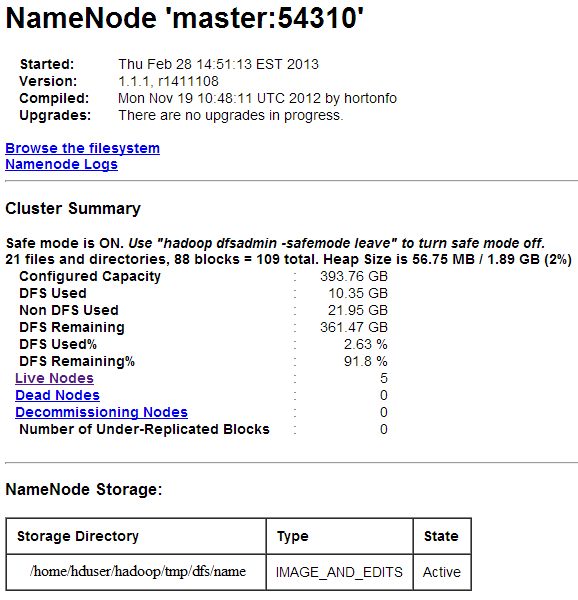
\includegraphics[width=.7\textwidth]{figs/5163os_04_08.png}
  \caption{Summary of a HDFS cluster}\label{fig:hdfs.summary}
\end{figure} 

By clicking on the Live Nodes link, we can check the status of each DataNode. We will get a web page similar to Figure \ref{fig:datanode.status}.
\begin{figure}[ht]
  \centering
  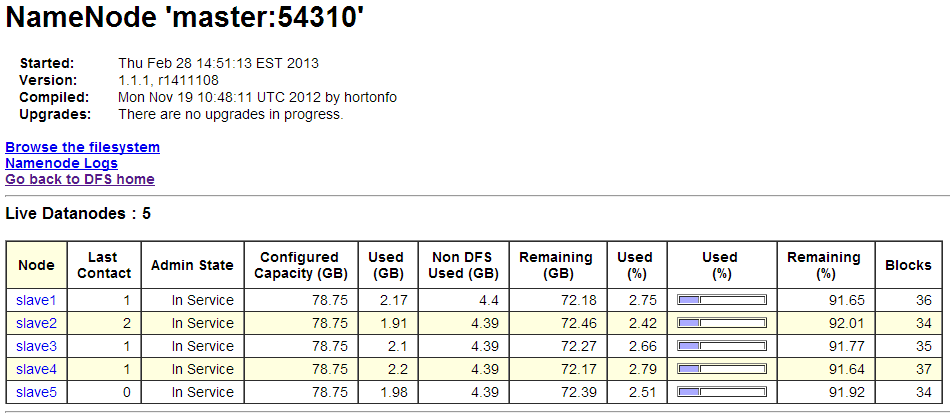
\includegraphics[width=.9\textwidth]{figs/5163os_04_09.png}
  \caption{HDFS DataNode status}\label{fig:datanode.status}
\end{figure} 

By clicking on the link of each node, we can browse the directory of the HDFS filesystem. The web page will be similar to Figure \ref{fig:content.hdfs}
\begin{figure}[ht]
  \centering
  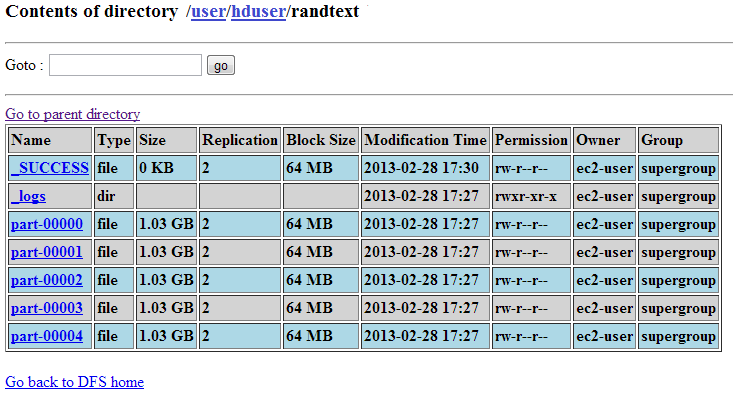
\includegraphics[width=.8\textwidth]{figs/5163os_04_10.png}
  \caption{Content of an HDFS directory}\label{fig:content.hdfs}
\end{figure} 

The web page shows that file \verb|/user/hduser/randtext| has been split into five partitions. We can browse the content of each partition by clicking on the \textbf{part-0000x} link.
\subsection*{See also}
\begin{itemize}
  \item The Validating Hadoop installation recipe in Chapter \ref{chap:3}, Configuring a Hadoop cluster
  \item The Decommissioning DataNode recipe
  \item The Manipulating files on HDFS recipe
\end{itemize}

\section{Configuring SecondaryNameNode}
Hadoop NameNode is a single point of failure. By configuring SecondaryNameNode\index{SecondaryNameNode}, the filesystem image and edit log\index{edit log} files can be backed up periodically. And in case of NameNode failure, the backup files can be used to recover the NameNode. In this recipe, we will outline steps to configure SecondaryNameNode.
\subsection*{Getting ready}
We assume that Hadoop has been configured correctly.\\
Log in to the master node from cluster administration machine using the following command:\\
\verb|$ ssh hduser@master|

\subsection*{How to do it...}
Perform the following steps to configure SecondaryNameNode: \\
Stop the cluster using the following command: \\
\verb|$ stop-all.sh|

Add or change the following into the file \verb|$HADOOP_HOME/conf/hdfs-site.xml|: 
\begin{verbatim}[language=XML]
<property>
    <name>fs.checkpoint.dir</name>
    <value>/hadoop/dfs/namesecondary</value>
</property>
\end{verbatim}

If this property is not set explicitly, the default checkpoint\index{checkpoint} directory will be \verb|${hadoop.tmp.dir}/dfs/namesecondary|.

Start the cluster using the following command: \\
\verb|$ start-all.sh|

The tree structure of NameNode data directory will be similar to the following:
\lstset{style=bashstyle}
\begin{lstlisting}
.
|-- current
|   |-- VERSION
|   |-- edits
|   |-- fsimage
|   `-- fstime
|-- image
|   `-- fsimage
|-- in_use.lock
`-- previous.checkpoint
    |-- VERSION
    |-- edits
    |-- fsimage
    `-- fstime

3 directories, 10 files
\end{lstlisting}

The tree structure of the SecondaryNameNode will be similar to that of the NameNode.

\subsection*{There's more...}
To increase redundancy\index{redundancy}, we can configure NameNode to write filesystem metadata\index{metadata} on multiple locations. For example, we can add an NFS\index{NFS} shared directory for backup by changing the following property in the file \verb|$HADOOP_HOME/conf/hdfs-site.xml|:
\lstset{style=bashstyle}
\begin{lstlisting}[language=XML]
<property>
  <name>dfs.name.dir</name>
  <value>/hadoop/dfs/name,/nfs/name</value>
</property>
\end{lstlisting}

\verb|/nfs/name| is an NFS shared directory on a remote machine.
\subsection*{See also}
\begin{itemize}
\item The Managing HDFS cluster recipe
\item The Decommissioning DataNode recipe
\end{itemize}
\section{Managing the MapReduce cluster}
A typical MapReduce cluster\index{MapReduce cluster} is composed of one master node that runs the JobTracker\index{JobTracker} and a number of slave nodes that run TaskTrackers\index{TaskTracker}. The task of managing a MapReduce cluster includes maintaining the health as well as the membership between TaskTrackers and the JobTracker. In this recipe, we will outline commands to manage a MapReduce cluster.
\subsection*{Getting ready}
We assume that the Hadoop cluster has been properly configured and running.
Log in to the master node from the cluster administration machine using the following command:
ssh hduser@master
\subsection*{How to do it...}
Perform the following steps to manage a MapReduce cluster:

List all the active TaskTrackers using the following command: \\
\verb|$ hadoop -job -list-active-trackers| \\
This command can help us check the registration status of the TaskTrackers in the cluster.

Check the status of JobTracker safe mode using the following command:
\lstset{style=bashstyle}
\begin{lstlisting}
$ hadoop mradmin -safemode get
Safe mode is OFF
\end{lstlisting}

The output tells us that the JobTracker is not in safe mode\index{safe mode}. We can submit jobs to the cluster. If the JobTracker is in safe mode, no jobs can be submitted to the cluster.

Manually let the JobTracker enter safe mode using the following command: \\
\verb|$ hadoop mradmin -safemode enter|

This command is handy when we want to maintain the cluster.

Let the JobTracker leave safe mode using the following command: \\
\verb|$ hadoop mradmin -safemode leave|

\begin{warning} When maintenance tasks are done, you need to run this command.\end{warning}

If we want to wait for safe mode to exit, the following command can be used: \\
\verb|$ hadoop mradmin -safemode wait|

Reload the MapReduce queue\index{queue} configuration using the following command: \\
\verb|$ hadoop mradmin -refreshQueues|

Reload active TaskTrackers using the following command:\\
\verb|$ hadoop mradmin -refreshNodes|

\subsection*{How it works...}
Get the help for the mradmin command using the following command:\index{hadoop mradmin}
\lstset{style=bashstyle}
\begin{lstlisting}
$ hadoop mradmin
The usage information will be similar to the following:
Usage: java MRAdmin
           [-refreshServiceAcl]
           [-refreshQueues]
           [-refreshUserToGroupsMappings]
           [-refreshSuperUserGroupsConfiguration]
           [-refreshNodes]
           [-safemode <enter | leave | get | wait>]
           [-help [cmd]]
...
\end{lstlisting}

The meaning of the command options is listed in Table \ref{tbl:mradmin}.
\begin{table}
  \centering
  \small
  \begin{tabular}{ll}
    \toprule 
    \textbf{Option} & \textbf{Description} \\  \midrule
    -refreshServiceAcl & Force JobTracker to reload service ACL. \\
    -refreshQueues & Force JobTracker to reload queue configurations. \\
    -refreshUserToGroupsMappings & Force JobTracker to reload user group mappings. \\
    -refreshSuperUserGroupsConfiguration & Force JobTracker to reload super user group mappings. \\
    -refreshNodes & Force JobTracker to refresh the JobTracker hosts. \\
    -help [cmd] & Show the help info for a command or all commands. \\ \bottomrule
  \end{tabular} 
  \caption{\textbf{mradmin} option description}\label{tbl:mradmin}
\end{table}

\subsection*{See also}
\begin{itemize}
\item The Configuring SecondaryNameNode recipe
\item The Managing MapReduce jobs recipe
\end{itemize} 

\section{Managing TaskTracker}\index{TaskTracker}
TaskTrackers are MapReduce daemon processes that run on slave nodes. They accept tasks assigned by the JobTracker on the master node and fork JVM processes/threads to run the tasks. TaskTracker is also responsible for reporting the progress of the tasks as well as its health status using heartbeat.

Hadoop maintains three lists for TaskTrackers: blacklist\index{blacklist}, gray list\index{gray list}, and excluded list\index{excluded list}. TaskTracker black listing is a function that can blacklist a TaskTracker if it is in an unstable state or its performance has been downgraded. For example, when the ratio of failed tasks\index{failed tasks} for a specific job has reached a certain threshold, the TaskTracker will be blacklisted for this job. Similarly, Hadoop maintains a gray list of nodes by identifying potential problematic nodes.

Sometimes, excluding certain TaskTrackers from the cluster is desirable. For example, when we debug or upgrade a slave node, we want to separate this node from the cluster in case it affects the cluster. Hadoop supports the live decommission\index{decommission} of a TaskTracker from a running cluster.

\subsection*{Getting ready}
We assume that Hadoop has been properly configured. MapReduce and HDFS daemons are running without any issues.

Log in to the cluster master node from the administrator machine using the following command: \\
\verb|$ ssh hduser@master|

List the active trackers with the following command on the master node:
\lstset{style=bashstyle}
\begin{lstlisting}
$ hadoop job -list-active-trackers
And the output should be similar to the following:
tracker_slave5:localhost/127.0.0.1:55590
tracker_slave1:localhost/127.0.0.1:47241
tracker_slave3:localhost/127.0.0.1:51187
tracker_slave4:localhost/127.0.0.1:60756
tracker_slave2:localhost/127.0.0.1:42939
\end{lstlisting}

\subsection*{How to do it...}
Perform the following steps to configure the heartbeat interval: 

Stop a MapReduce cluster with the following command:\\
\verb|$ stop-dfs.sh|

Open the file \verb|$HADOOP_HOME/conf/mapred-site.xml| with your favorite text editor and add the following content into the file:
\lstset{style=bashstyle}
\begin{lstlisting}[language=XML]
<property>
  <name>mapred.tasktracker.expiry.interval</name>
  <value>600000</value>
</property>
\end{lstlisting}

The value is in milliseconds.

Copy the configuration into the slave nodes using the following command:
\lstset{style=bashstyle}
\begin{lstlisting}[language=bash]
for host in `cat $HADOOP_HOME/conf/slaves`; do
  echo 'Copying mapred-site.xml to slave node ' $host
  sudo scp $HADOOP_HOME/conf/mapred-site.xml hduser@$host:$HADOOP_HOME/conf
done
\end{lstlisting}

Start the MapReduce cluster with the following command: \\
\verb|$ start-mapred.sh|

Perform the following steps to configure TaskTracker blacklisting:

Stop the MapReduce cluster with the following command: \\
\verb|$ stop-mapred.sh|

Set the number of task failures for a job to blacklist a TaskTracker by adding or changing the following property in the file \verb|$HADOOP_HOME/conf/hdfs-site.xml|:
\lstset{style=bashstyle}
\begin{lstlisting}[language=XML]
<property>
  <name>mapred.max.tracker.failures</name>
  <value>10</value>
</property>
\end{lstlisting}

Set the maximum number of successful jobs that can blacklist a TaskTracker by adding or changing the following property in the file \verb|$HADOOP_HOME/conf/hdfs-site.xml|:
\lstset{style=bashstyle}
\begin{lstlisting}[language=XML]
<property>
  <name>mapred.max.tracker.blacklists</name>
  <value>5</value>
</property>
\end{lstlisting}

Copy the configuration file to the slave nodes using the following commands:
\lstset{style=bashstyle}
\begin{lstlisting}[language=bash]
for host in `cat $HADOOP_HOME/conf/slaves`; do
  echo 'Copying hdfs-site.xml to slave node ' $host
  sudo scp $HADOOP_HOME/conf/hdfs-site.xml hduser@$host:$HADOOP_HOME/conf
done
\end{lstlisting}

Start the MapReduce cluster using the following command: \\
\verb|$ start-mapred.sh|

List blacklisted TaskTrackers using the following command: \\
\verb|$ hadoop job -list-blacklisted-trackers|

Perform the following steps to decommission TaskTrackers: 

Set the TaskTracker exclude file\index{TaskTracker exclude file} by adding the following properties into the file:
\lstset{style=bashstyle}
\begin{lstlisting}[language=XML]
<property>
  <name>mapred.hosts.exclude</name>
  <value>$HADOOP_HOME/conf/mapred-exclude.txt</value>
</property>
\end{lstlisting}

The \verb|$HADOOP_HOME/conf/mapred-exclude.txt| file will contain the excluding TaskTracker hostnames one per line. For example, the file should contain the following two lines if we want to exclude \emph{slave1} and \emph{slave3} from the cluster: 
\lstset{style=bashstyle}
\begin{lstlisting}
slave1
slave3
\end{lstlisting}

Force the JobTracker to reload the TaskTracker list with the following command: \\
\verb|$ hadoop mradmin -refreshNodes|

List all the active trackers again using the following command:
\lstset{style=bashstyle}
\begin{lstlisting}
$ hadoop job -list-active-trackers
tracker_slave5:localhost/127.0.0.1:55590
tracker_slave4:localhost/127.0.0.1:60756
tracker_slave2:localhost/127.0.0.1:42939
\end{lstlisting}

\subsection*{How it works...}
TaskTrackers on slave nodes contact the JobTracker on the master node periodically. The interval between two consecutive contact communications is called a heartbeat\index{hearbeat}. More frequent heartbeat configurations can incur higher load to the cluster. The value of the heartbeat property should be set based on the size of the cluster.

The JobTracker uses TaskTracker blacklisting to remove those unstable TaskTrackers. If a TaskTracker is blacklisted, all the tasks currently running on the TaskTracker can still finish and the TaskTracker will continue the connection with JobTracker through the heartbeat mechanism. But the TaskTracker will not be scheduled for running future tasks. If a blacklisted TaskTracker is restarted, it will be removed from the blacklist.

The total number of blacklisted TaskTrackers should not exceed 50 percent of the total number of TaskTrackers.
\subsection*{See also}
\begin{itemize}
  \item The Managing the MapReduce cluster recipe
  \item The Managing MapReduce jobs recipe
  \item The Decommissioning DataNode recipe
  \item The Replacing a slave node recipe
\end{itemize}

\section{Decommissioning DataNode}
Similar to TaskTracker, there are situations when we need to temporarily disable a DataNode from the cluster, for example, because the storage space of the DataNode has been used up. In this recipe, we will outline steps to decommission a DataNode\index{decommission DataNode} from a live Hadoop cluster.
\subsection*{Getting ready}
We assume that our Hadoop has been configured properly.

Log in to the master node from the cluster administrator machine with the following command: \\
\verb|$ ssh hduser@master|

For illustration purpose, we assume to decommission DataNode on host slave1 from our running Hadoop cluster.
\subsection*{How to do it...}
Perform the following steps to decommission a live DataNode:

Create the file \verb|$HADOOP_HOME/conf/dfs-exclude.txt| with the following content:\\
\verb|slave1|

The \verb|dfs-exclude.txt| file contains the DataNode hostnames, one per line, that are to be decommissioned from the cluster.

Add the following property to the file \verb|$HADOOP_HOME/conf/hdfs-site.xml|:
\lstset{style=bashstyle}
\begin{lstlisting}[language=XML]
<property>
  <name>dfs.hosts.exclude</name>
  <value>$HADOOP_HOME/conf/dfs-exclude.txt</value>
</property>
\end{lstlisting}

Force the NameNode to reload the active DataNodes using the following command: \\
\verb|$ hadoop dfsadmin -refreshNodes|

Get a description report of each active DataNode: \\
\verb|$ hadoop dfsadmin -report|

\subsection*{How it works...}
Cluster administrators can use the dfsadmin command to manage the DataNodes. We can get the usage of this command using the following:\index{hadoop dfsadmin}
\lstset{style=bashstyle}
\begin{lstlisting}
$ hadoop dfsadmin
Usage: java DFSAdmin
           [-report]
           [-safemode enter | leave | get | wait]
           [-saveNamespace]
           [-refreshNodes]
           [-finalizeUpgrade]
           [-upgradeProgress status | details | force]
           ...
\end{lstlisting}
\subsection*{See also}
\begin{itemize}
  \item The Managing the HDFS cluster recipe
  \item The Configuring SecondaryNameNode recipe
  \item The Managing TaskTracker recipe
  \item The Replacing a slave node recipe
\end{itemize}

\section{Replacing a slave node}
Sometimes, we need to replace a slave node with new hardware, because of reasons such as the slave node is not stable, more storage space or more powerful CPUs are desired, and so on. In this recipe, we will outline the steps to replace a slave node.

\subsection*{Getting ready}
We assume that replacement hardware is ready for use. And for illustration purposes, we suppose \emph{slave2} needs to be replaced in this book.

\subsection*{How to do it...}\index{decommission}
Perform the following steps to replace a slave node:

Decommission the TaskTracker on the slave node with the steps outlined in the Managing TaskTracker recipe of this chapter. 

Decommission the DataNode on the slave node with the steps outlined in the Decommission DataNode recipe of this chapter. 

Power off the slave node and replace it with the new hardware.

Install and configure the Linux operating system on the new node with the steps outlined in the Installing the Linux operating system, Installing Java and other tools, and Configuring SSH recipes of Chapter 2, Preparing for Hadoop Installation.

Install Hadoop on the new node by copying the Hadoop directory and configuration from the master node with the following commands:
\lstset{style=bashstyle}
\begin{lstlisting}[language=bash]
$ sudo scp -r /usr/local/hadoop-1.1.2 hduser@slave2:/usr/local/
$ sudo ssh hduser@slave2 -C "ln -s /usr/local/hadoop-1.1.2 /usr/local/hadoop"
$ sudo scp ~/.bashrc hduser@slave2:~/
\end{lstlisting}

Log in to \verb|slave2| and start the DataNode and TaskTracker using the following commands: 
\lstset{style=bashstyle}
\begin{lstlisting}[language=bash]
$ ssh hduser@slave2 -C "hadoop DataNode &"
$ ssh hduser@slave2 -C "Hadoop TaskTracker &" 
\end{lstlisting}

Refresh the DataNodes with the following command: \\
\verb|$ hadoop dfsadmin -refreshNodes|

Refresh the TaskTracker with the following command: \\
\verb|$ hadoop mradmin -refreshNodes|

Report the status of the live DataNodes with the following command: \\
\verb|$ hadoop dfsadmin -report|

Get all the active TaskTrackers with the following command: \\
\verb|$ hadoop job -list-active-trackers|
\subsection*{See also}
\begin{itemize}
  \item The Installing Linux on node recipe of Chapter \ref{chap:2}, Preparing for Hadoop Installation
  \item The Installing Java and other tools recipe of Chapter \ref{chap:2}, Preparing for Hadoop Installation
  \item The Configuring SSH recipe of Chapter \ref{chap:2}, Preparing for Hadoop installation
  \item The Configuring Hadoop in Fully-distributed Mode recipe of Chapter \ref{chap:3}, Configuring a Hadoop Cluster
  \item The Managing TaskTracker recipe
  \item The Decommissioning DataNode recipe
\end{itemize}

\section{Managing MapReduce jobs}\index{MapReduce jobs}
The Hadoop Big Data platform accepts jobs submitted by clients. In a multiuser environment, multiple jobs can be submitted and run simultaneously. The tasks of managing Hadoop jobs include checking job status, changing job priority, killing a running job, and so on. In this recipe, we will outline the steps to do these job management tasks.
\subsection*{Getting ready}
We assume that our Hadoop cluster has been configured properly and all the Hadoop daemons are running without any issues. We also assume that a regular user can submit Hadoop jobs to the cluster.

Log in to the master node from the cluster administrator machine with the following command:\\
\verb|$ ssh hduser@master|
\subsection*{How to do it...}
Perform the following steps to check the status of Hadoop jobs:

List all the running jobs using the following command: 
\lstset{style=bashstyle}
\begin{lstlisting}
$ hadoop job -list
1 jobs currently running
JobId   State   StartTime   UserName        Priority        SchedulingInfo
job_201302152353_0001   4   1361405786524   hduser  NORMAL  NA
\end{lstlisting}

The output message tells us that currently one job with JobId \verb|job_201302152353_0001| is running on the cluster.

List all the submitted jobs since the start of the cluster with the following command: 
\lstset{style=bashstyle}
\begin{lstlisting}
hadoop job -list all
2 jobs submitted
States are:
  Running : 1     Succeded : 2    Failed : 3      Prep : 4
JobId   State   StartTime   UserName        Priority        SchedulingInfo
job_201302152353_0001   2   1361405786524   hduser  NORMAL  NA
job_201302152353_0002   4   1361405860611   hduser  NORMAL  NA
\end{lstlisting}

The State column of the output message shows the status of jobs. For example, in the preceding output, two jobs have been submitted, the first job with JobId \verb|job_201302152353_0001| is in the succeeded state and the second job with JobId \verb|job_201302152353_0002| is in the preparation state. Both jobs have normal priority and don't have scheduling information.

We can check the status of the default queue with the following command:
\begin{verbatim}
$ hadoop queue -list
Queue Name : default
Queue State : running
Scheduling Info : N/A
\end{verbatim}

Hadoop manages jobs using queues. By default, there is only one default queue. The output of the command shows the cluster has only one default queue, which in the running state with no scheduling information.

Check the status of a queue ACL with the following command: 
\begin{verbatim}
$ hadoop queue -showacls
Queue acls for user :  hduser

Queue  Operations
=====================
default  submit-job,administer-jobs
\end{verbatim}

The output shows that the user hduser can submit and administer jobs in the default queue.

Show all the jobs in the default queue using the following command:
\lstset{style=bashstyle}
\begin{lstlisting}
$ hadoop queue -info default -showJobs
Queue Name : default
Queue State : running
Scheduling Info : N/A
Job List
JobId   State   StartTime   UserName   Priority   SchedulingInfo
job_201302152353_0001   2   1361405786524   hduser  NORMAL  NA
\end{lstlisting}

Check the status of a job with the following command:
\lstset{style=bashstyle}
\begin{lstlisting}
$ hadoop job -status job_201302152353_0001
Job: job_201302152353_0001
file: hdfs://master:54310/user/hduser/.staging/job_201302152353_0001/job.xm                l
tracking URL: http://master:50030/jobdetails.jsp?jobid=job_201302152353_000                1
map() completion: 1.0
reduce() completion: 1.0

Counters: 31
        Job Counters
                Launched reduce tasks=1
                SLOTS_MILLIS_MAPS=87845
                Total time spent by all reduces waiting after reserving slots (ms)=0
                Total time spent by all maps waiting after reserving slots (ms)= 0
                Rack-local map tasks=8
                Launched map tasks=10
                Data-local map tasks=2
                SLOTS_MILLIS_REDUCES=16263
        File Input Format Counters
                Bytes Read=1180
        File Output Format Counters
                Bytes Written=97
        FileSystemCounters
                FILE_BYTES_READ=226
                HDFS_BYTES_READ=2440
                FILE_BYTES_WRITTEN=241518
                HDFS_BYTES_WRITTEN=215
        Map-Reduce Framework
                Map output materialized bytes=280
                Map input records=10
                Reduce shuffle bytes=252
                Spilled Records=40
                Map output bytes=180
                Total committed heap usage (bytes)=2210988032
                CPU time spent (ms)=9590
                Map input bytes=240
                SPLIT_RAW_BYTES=1260
                Combine input records=0
                Reduce input records=20
                Reduce input groups=20
                Combine output records=0
                Physical memory (bytes) snapshot=2033074176
                Reduce output records=0
                Virtual memory (bytes) snapshot=5787283456
                Map output records=20
\end{lstlisting}

Change the status of a job by performing the following steps:  

Set the job \verb|job_201302152353_0001| to be on high priority using the following command: \\
\verb|$ hadoop job -set-priority job_201302152353_0003 HIGH|

Available priorities, in descending order, include: \verb|VERY_HIGH, HIGH, NORMAL, LOW|, and \verb|VERY_LOW|.

The priority of the job will\index{job priority} be \emph{HIGH} as shown in the following output:
\lstset{style=bashstyle}
\begin{lstlisting}
4 jobs submitted
States are:
        Running : 1     Succeded : 2    Failed : 3      Prep : 4
JobId   State   StartTime   UserName        Priority        SchedulingInfo
job_201302152353_0001   2   1361405786524   hduser  NORMAL  NA
job_201302152353_0002   2   1361405860611   hduser  NORMAL  NA
job_201302152353_0003   1   1361408177470   hduser  HIGH    NA
\end{lstlisting}

Kill the job\index{kill job} \verb|job_201302152353_0004| using the following command: \\
\verb|$ hadoop job -kill job_201302152353_0004|

With the job status command, we will get the following output:
\lstset{style=bashstyle}
\begin{lstlisting}
3 jobs submitted
States are:
 Running : 1   Succeded : 2  Failed : 3   Prep : 4   Killed : 5
JobId   State   StartTime   UserName        Priority        SchedulingInfo
job_201302152353_0001   2   1361405786524   hduser  NORMAL  NA
job_201302152353_0002   2   1361405860611   hduser  NORMAL  NA
job_201302152353_0003   1   1361408177470   hduser  HIGH    NA
job_201302152353_0004   5   1361407740639   hduser  NORMAL  NA
\end{lstlisting}

\begin{info}
The Killed : 5 information is not in the original output, I put it there according to the state of the killed job \verb|job_201302152353_0004|.
\end{info}

Perform the following steps to submit a MapReduce job:

Create the job configuration file, \emph{job.xml}, with the following content:
\lstset{style=bashstyle}
\begin{lstlisting}[language=XML]
<?xml version="1.0" encoding="UTF-8" standalone="no"?>
<configuration>
  <property>
    <name>mapred.input.dir</name>
    <value>randtext</value>
  </property>

  <property>
    <name>mapred.output.dir</name>
    <value>output</value>
  </property>

  <property>
    <name>mapred.job.name</name>
    <value>wordcount</value>
  </property>

  <property>
    <name>mapred.mapper.class</name>
    <value>org.apache.hadoop.mapred.WordCount$Map</value>
  </property>

  <property>
    <name>mapred.combiner.class</name>
    <value>org.apache.hadoop.mapred.WordCount$Reduce</value>
  </property>

  <property>
    <name>mapred.reducer.class</name>
    <value>org.apache.hadoop.mapred.WordCount$Reduce</value>
  </property>

  <property>
    <name>mapred.input.format.class</name>
    <value>org.apache.hadoop.mapred.TextInputFormat</value>
  </property>

  <property>
    <name>mapred.output.format.class</name>
    <value>org.apache.hadoop.mapred.TextOutputFormat</value>
  </property>

</configuration>
\end{lstlisting}
The \emph{job.xml} file is an XML file that specifies the configuration of a job. In this job configuration file, we specified the job name, the mapper class, the reducer class, the combiner class, the input format, and output format for the job. We have used wordcount as an example, so we also need to make sure \verb|$HADOOP_HOME/hadoop-examples*.jar| is available in \verb|CLASSPATH|.

Submit the job with the following command:
\lstset{style=bashstyle}
\begin{lstlisting}
$ hadoop job -submit job.xml
13/03/01 11:55:53 WARN mapred.JobClient: Use GenericOptionsParser for parsing the arguments. Applications should implement Tool for the same.
13/03/01 11:55:53 INFO util.NativeCodeLoader: Loaded the native-hadoop library
13/03/01 11:55:53 WARN snappy.LoadSnappy: Snappy native library not loaded
13/03/01 11:55:53 INFO mapred.FileInputFormat: Total input paths to process : 5
Created job job_201302281451_0012
\end{lstlisting}
\subsection*{How it works...}
The queue command is a wrapper command for the JobQueueClient class, and the job command is a wrapper command for the JobClient class.

We can get the usage of the queue command with the following:\index{hadoop queue}
\lstset{style=bashstyle}
\begin{lstlisting}
$ hadoop queue
Usage: JobQueueClient <command> <args>
        [-list]
        [-info <job-queue-name> [-showJobs]]
        [-showacls]
\end{lstlisting}

Similarly, we can get the usage of the job command with the following: \index{hadoop job}
\lstset{style=bashstyle}
\begin{lstlisting}
$ hadoop job
Usage: JobClient <command> <args>
        [-submit <job-file>]
        [-status <job-id>]
        [-counter <job-id> <group-name> <counter-name>]
        [-kill <job-id>]
        [-set-priority <job-id> <priority>]. Valid values for priorities are: VERY_HIGH HIGH NORMAL LOW VERY_LOW
        [-events <job-id> <from-event-#> <#-of-events>]
        [-history <jobOutputDir>]
        [-list [all]]
        [-list-active-trackers]
        [-list-blacklisted-trackers]
        [-list-attempt-ids <job-id> <task-type> <task-state>]
        [-kill-task <task-id>]
        [-fail-task <task-id>]
\end{lstlisting}
\subsection*{There's more...}
We discussed the most useful commands for Hadoop job management. Actually, there are even more commands that are related to job management, and alternatively, we can use the web UI to manage Hadoop jobs.

\subsubsection*{More job management commands}
Get the value of a counter: \\
\verb|$ hadoop job -counter <job-id> <group-name> <counter-name>|

For example, we can get the counter \verb|HDFS_BYTES_WRITTEN| of the counter group FileSystemCounters\index{FileSystemCounters} for the job \verb|job_201302281451_0002| with the following command: 
\lstset{style=bashstyle}
\begin{lstlisting}[language=bash]
$ hadoop job -counter job_201302281451_0002 FileSystemCounters HDFS_BYTES_WRITTEN
\end{lstlisting}

Query events of a MapReduce job with the following command: \\
\verb|$ hadoop job -events <job-id> <from-event-#> <#-of-events>|

For example, we can query the first 10 events of the job \verb|job_201302281451_0002| using the following command: \\
\verb|$ hadoop job -events job_201302281451_0002 0 10|

We will get output similar to Figure \ref{fig:task.events}.
\begin{figure}[ht]
  \centering
  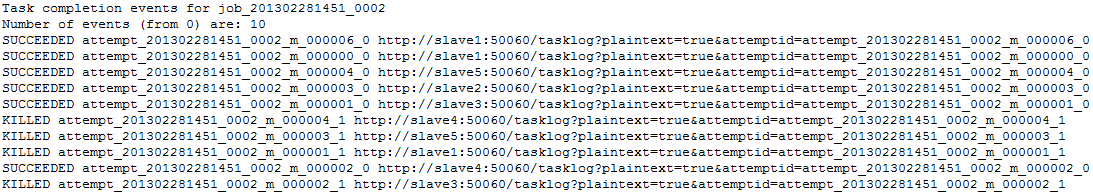
\includegraphics[width=\textwidth]{figs/5163os_04_13.png}
  \caption{MapReduce task completion events}\label{fig:task.events}
\end{figure} 

Get the job history\index{job history} including job details, failed and killed jobs, and so on with the following command: 
\lstset{style=bashstyle}
\begin{lstlisting}
$hadoop job -history
Hadoop job: 0012_1362156954465_hduser
=====================================
Job tracker host name: job
job tracker start time: Tue May 18 17:18:01 EDT 1976
User: hduser
JobName: wordcount
JobConf: hdfs://master:54310/user/hduser/.staging/job_201302281451_0012/job.xml
Submitted At: 1-Mar-2013 11:55:54
Launched At: 1-Mar-2013 11:55:54 (0sec)
Finished At: 1-Mar-2013 11:56:43 (48sec)
Status: FAILED
Counters:

|Group Name |Counter name|Map Value |Reduce Value |Total Value|
-------------------------------------------------------
=====================================

Task Summary
============================
Kind Total Successful Failed Killed StartTime   FinishTime

Setup 1 1 0 0 1-Mar-2013 11:55:46  1-Mar-2013 11:55:49 (2sec)
Map 45 0 38 7 1-Mar-2013 11:55:49  1-Mar-2013 11:56:34 (44sec)
Reduce  0   0   0   0
Cleanup 1 1 0 0 1-Mar-2013 11:56:33 1-Mar-2013 11:56:36 (3sec)
============================

No Analysis available as job did not finish

KILLED SETUP task list for 0012_1362156954465_hduser
TaskId          StartTime       FinishTime      Error
====================================================

FAILED MAP task list for 0012_1362156954465_hduser
TaskId          StartTime       FinishTime      Error   InputSplits
====================================================
task_201302281451_0012_m_000000 1-Mar-2013 11:55:58  1-Mar-2013 11:56:33 (35sec)  /default-rack/slave2,/default-rack/slave1

...
FAILED task attempts by nodes
Hostname        FailedTasks
===============================
slave1  task_201302281451_0012_m_000000, task_201302281451_0012_m_000001, task_201302281451_0012_m_000002, task_201302281451_0012_m_000004, task_201302281451_0012_m_000005, task_201302281451_0012_m_000008, task_201302281451_0012_m_000010, task_201302281451_0012_m_000013,
slave2  task_201302281451_0012_m_000000, task_201302281451_0012_m_000005, task_201302281451_0012_m_000008, task_201302281451_0012_m_000010, task_201302281451_0012_m_000019, task_201302281451_0012_m_000034, task_201302281451_0012_m_000036, task_201302281451_0012_m_000039,
slave3  task_201302281451_0012_m_000000, task_201302281451_0012_m_000001, task_201302281451_0012_m_000002, task_201302281451_0012_m_000003, task_201302281451_0012_m_000004, task_201302281451_0012_m_000010, task_201302281451_0012_m_000012, task_201302281451_0012_m_000019,
slave4  task_201302281451_0012_m_000000, task_201302281451_0012_m_000001, task_201302281451_0012_m_000003, task_201302281451_0012_m_000004, task_201302281451_0012_m_000010, task_201302281451_0012_m_000012, task_201302281451_0012_m_000013, task_201302281451_0012_m_000034,
slave5  task_201302281451_0012_m_000002, task_201302281451_0012_m_000003, task_201302281451_0012_m_000005, task_201302281451_0012_m_000008, task_201302281451_0012_m_000012, task_201302281451_0012_m_000013,

KILLED task attempts by nodes
Hostname        FailedTasks
===============================
slave1  task_201302281451_0012_m_000003, task_201302281451_0012_m_000012,
slave2  task_201302281451_0012_m_000002, task_201302281451_0012_m_000013,
slave3  task_201302281451_0012_m_000005,
slave5  task_201302281451_0012_m_000001, task_201302281451_0012_m_000004,
\end{lstlisting}

\section{Managing tasks}
We will show you how to kill tasks, check task attempts, and so on. 

Kill a task with the following command:\index{kill task} \\
\verb|$ hadoop job -kill-task <task-id> |

For example, to kill the task \verb|task_201302281451_0013_m_000000|, we can use the following command: \\ 
\verb|$ hadoop job -kill-task task_201302281451_0013_m_000000|

After the task is killed, the JobTracker will restart the task on a different node. The killed tasks can be viewed through the web UI as shown in Figure \ref{fig:mapred.killed.tasks}.
\begin{figure}[ht]
  \centering
  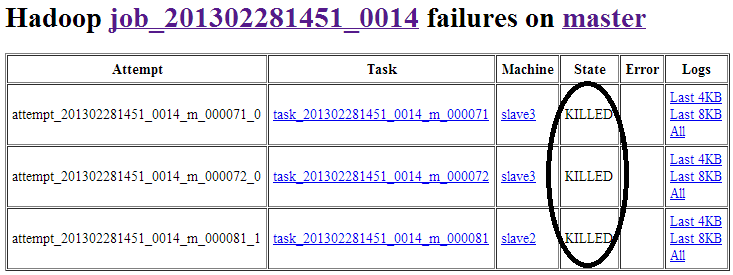
\includegraphics[width=\textwidth]{figs/5163os_04_14.png}
  \caption{Status of killed tasks}\label{fig:mapred.killed.tasks}
\end{figure} 
Hadoop JobTracker can automatically kill tasks in the following situations:
\begin{itemize}
  \item A task does not report progress after timeout
  \item Speculative execution can run one task on multiple nodes, if one of these task is succeeded, other attempts of the same task will be killed, because the attempt results for those attempts will be useless
  \item Job/Task schedulers such as fair scheduler and capacity scheduler need empty slots for other pools or queues
\end{itemize}

In many situations, we need a task to fail, which can be done with the following command: \\
\verb|$ hadoop job -fail-task <task-id> |\index{hadoop job -fail-task}

For example, to fail the task \verb|task_201302281451_0013_m_000000|, we can use the following command:
\lstset{style=bashstyle}
\begin{lstlisting}[language=bash]
$ hadoop job -fail-task task_201302281451_0013_m_000000
\end{lstlisting}

List task attempts with the following command:
\lstset{style=bashstyle}
\begin{lstlisting}[language=bash]
$ hadoop job -list-attempt-ids <job-id> <task-type> <task-state>
\end{lstlisting}

In this command, available task types are \emph{map, reduce, setup}, and \emph{clean}; available task states are running and completed.
For example, to list all the completed map attempts for the job \verb|job_201302281451_0014|, the following command can be used: 
\lstset{style=bashstyle}
\begin{lstlisting}
$ hadoop job -list-attempt-ids job_201302281451_0014 map completed
attempt_201302281451_0014_m_000000_0
attempt_201302281451_0014_m_000001_0
attempt_201302281451_0014_m_000002_0
attempt_201302281451_0014_m_000009_0
attempt_201302281451_0014_m_000010_0
...
\end{lstlisting}

\section{Managing jobs through the web UI}
We will show job management from the web UI.

Check the status of a job by opening the JobTracker URL: \url{master:50030/jobtracker.jsp}.

We will get a web page similar to Figure \ref{fig:mapred.status}.
\begin{figure}[ht]
  \centering
  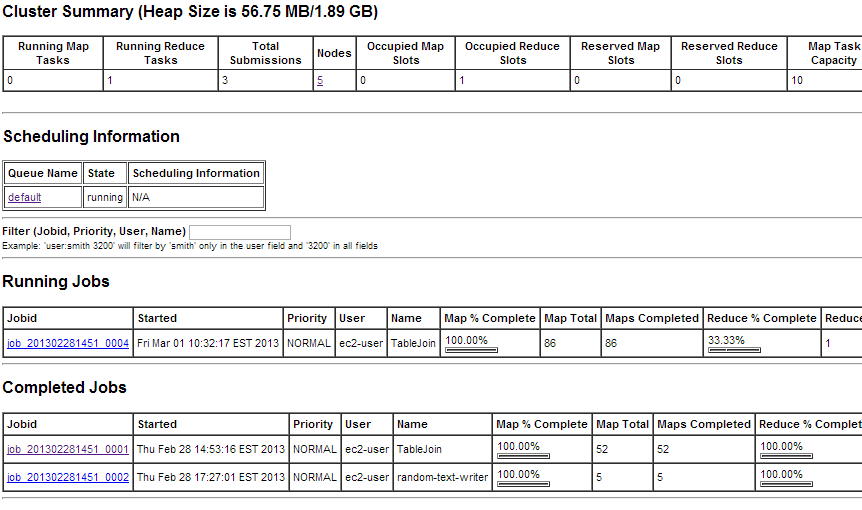
\includegraphics[width=\textwidth]{figs/5163os_04_11.png}
  \caption{MapReduce Job and Scheduling information}\label{fig:mapred.status}
\end{figure} 
From this web page, we can get the cluster summary information, the scheduling information, the running jobs list, the completed jobs list, and the retired jobs list. By clicking on a specific job link, we can check the details of a job, or we can open the URL, \url{http://master:50030/jobdetails.jsp?jobid=job_201302281451_0004&refresh=30}. By specifying the refresh parameter, we can tell the web page to refresh every 30 seconds.

Kill a job by opening the URL, \url{master:50030/jobdetails.jsp?jobid=job_201302281451_0007&action=kill}.

After a while, the killed job will be listed in the Failed Jobs list as shown in Figure \ref{fig:failed.job}.
\begin{figure}[ht]
  \centering
  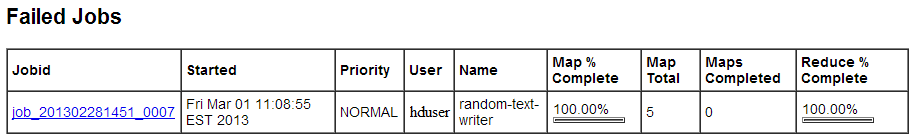
\includegraphics[width=\textwidth]{figs/5163os_04_12.png}
  \caption{Information of a Failed job}\label{fig:failed.job}
\end{figure} 

Change the job priority to be HIGH by opening the URL, \url{master:50030/jobdetails.jsp?jobid=job_201302281451_0007&action=changeprio&prio=HIGH}. \\
\subsection*{See also}
\begin{itemize}
  \item The Validating Hadoop installation recipe of Chapter \ref{chap:3}, Configuring a Hadoop Cluster
  \item The Managing the HDFS cluster recipe
  \item The Managing MapReduce cluster recipe
  \item Refer to \href{http://hadoop.apache.org/docs/r1.1.2/mapred_tutorial.html}{MapReduce tutorial}.
\end{itemize}

\section{Checking job history from the web UI}
Hadoop keeps track of all the submitted jobs in the logs directory. The job history\index{job history} logs contain information for each job such as the total run time and the run time of each task. In this section, we will show you how to check the job history logs through a web UI.
\subsection*{Getting ready}
We assume that our Hadoop cluster has been properly configured and all daemons are running without any issues.
\subsection*{How to do it...}
Perform the following steps to check job history logs from web UI:

Open the job history URL, \url{http://master:50030/jobhistoryhome.jsp}. \\
We will be able to get a web page similar to Figure \ref{fig:history.jobs}
\begin{figure}[ht]
  \centering
  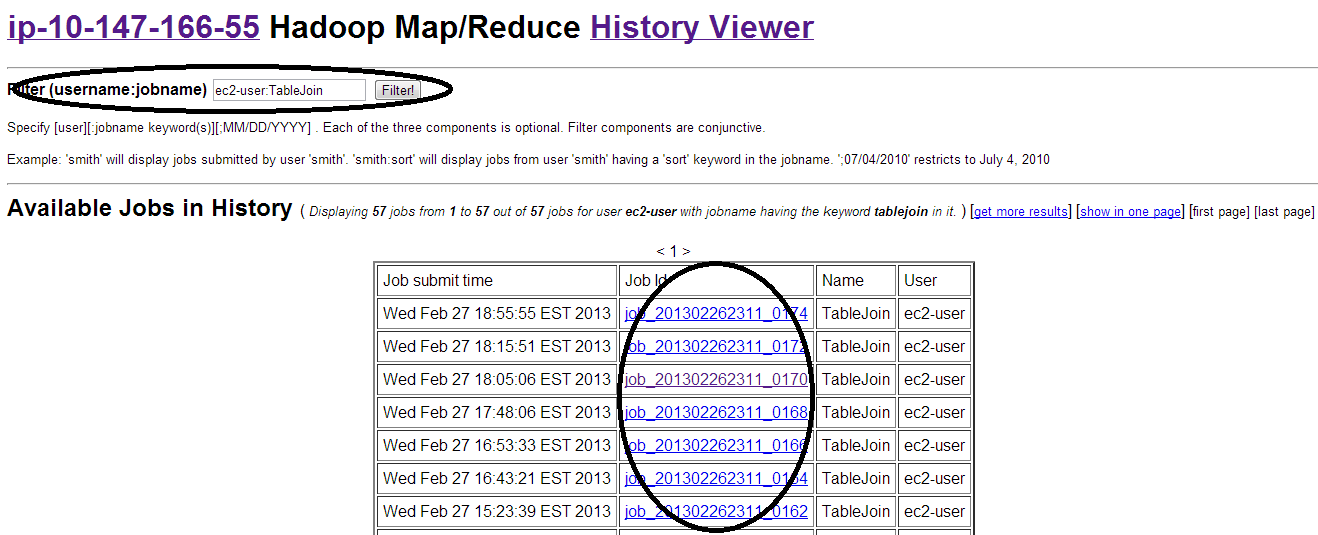
\includegraphics[width=\textwidth]{figs/5163os_04_01.png}
  \caption{History jobs}\label{fig:history.jobs}
\end{figure} 

On the web UI, we can filter jobs based on the username and job name in the format \textbf{username:jobname} as shown in Figure \ref{fig:history.jobs}. username should be the username that runs a certain job, and job name should contain keywords of Hadoop jobs.

From the web UI, we will be able to get a list of jobs in the Available Jobs in History section. By clicking on the Job Id link of a job, we can get the details of the job as shown in Figure \ref{fig:specific.job.history}.
\begin{figure}[ht]
  \centering
  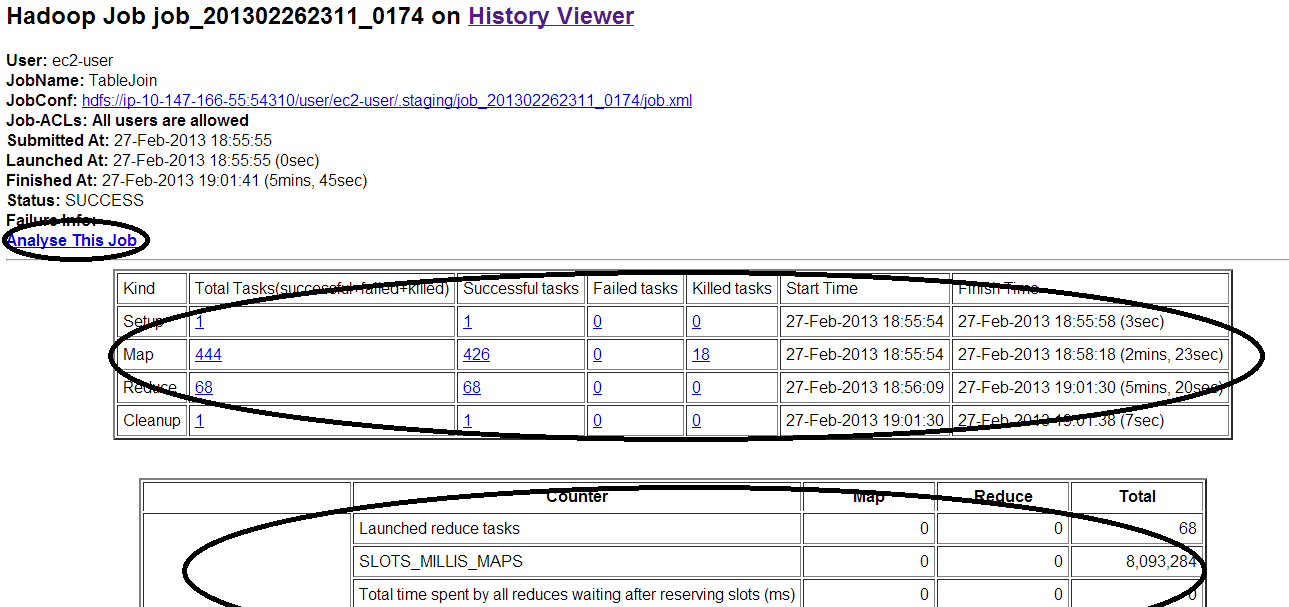
\includegraphics[width=\textwidth]{figs/5163os_04_02.png}
  \caption{History of a specific job}\label{fig:specific.job.history}
\end{figure} 
This web page shows the details of the job, including task information such as total, successful, failed, and killed tasks. The information also includes the start time and end time of four phases of a Hadoop job including setup, map, reduce, and cleanup phases.

The web page also contains information of counters of the job as shown in the lower part of Figure \ref{fig:specific.job.history}.

In addition to the summary of job information, the web UI provides interface for us to analyze a job. By clicking on the link \emph{Analyze This Job}, we will go to a web page similar to Figure \ref{fig:task.statistics}.\index{taks statistics}
\begin{figure}[ht]
  \centering
  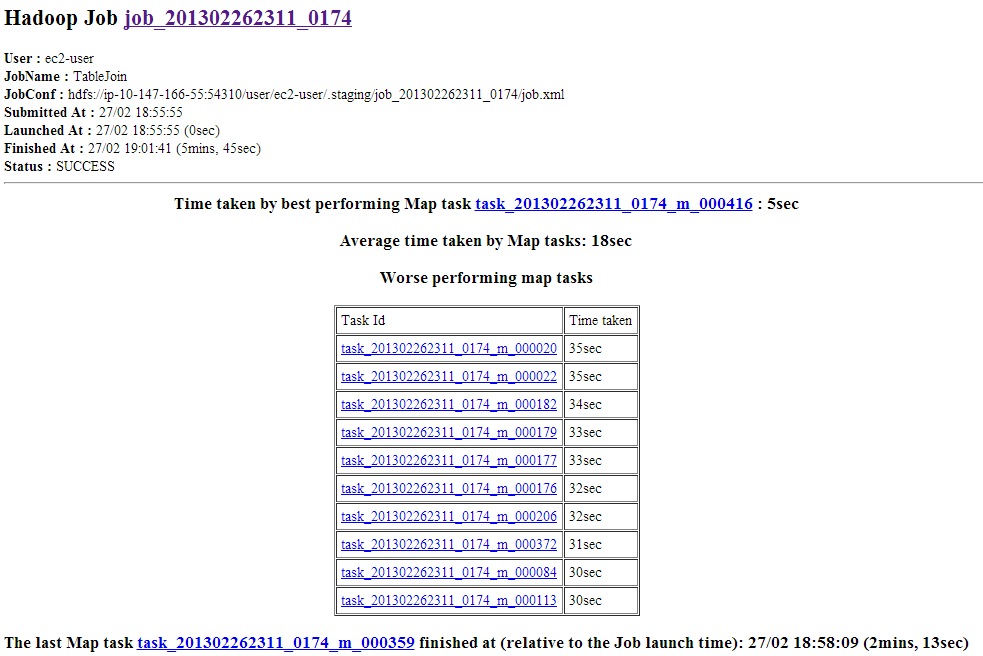
\includegraphics[width=\textwidth]{figs/5163os_04_03.png}
  \caption{Statistics of tasks for a job}\label{fig:task.statistics}
\end{figure} 
The web page contains information of simple time analytics for each task, for example the best performing tasks that take the shortest time, the worse performing tasks, and the average time taken by all the tasks.

To further check the information of a task, we can click on the link for the task, and we will get a web page similar to Figure \ref{fig:task.info}.
\begin{figure}[ht]
  \centering
  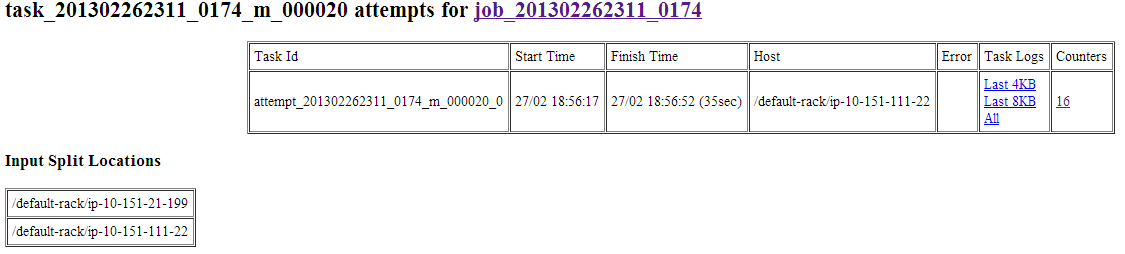
\includegraphics[width=.7\textwidth]{figs/5163os_04_04.png}
  \caption{Information of a task}\label{fig:task.info}
\end{figure} 
We can get the counters of a task by clicking on the Counters field of the task as shown in Figure \ref{fig:task.info}, or we can get the same web page by opening URL \url{http://master:50030/taskstats.jsp?tipid=task_201302281211_0001_m_000000}.

In this URL, \verb|task_201302281211_0001_m_000000| is the task ID we want to get counters for.

We will be able to get task counters as shown in Figure \ref{fig:task.counters}
\begin{figure}[ht]
  \centering
  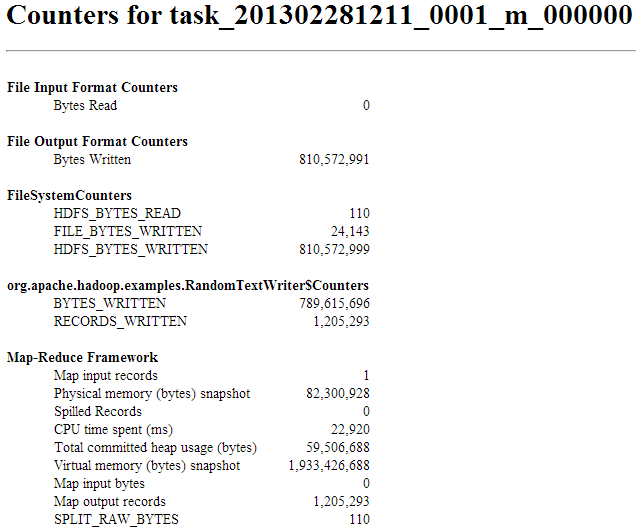
\includegraphics[width=.8\textwidth]{figs/5163os_04_05.png}
  \caption{Task Counters}\label{fig:task.counters}
\end{figure} 
In addition to all these web services, the web UI provides a graphical display of the progress of Hadoop jobs and each phase as shown in Figure \ref{fig:mapreduce.progress}.
\begin{figure}[ht]
  \centering
  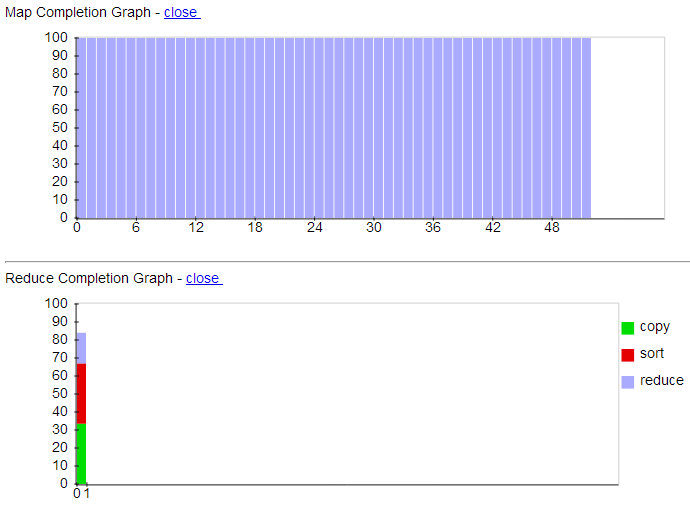
\includegraphics[width=.8\textwidth]{figs/5163os_04_06.png}
  \caption{Progress of map and reduce tasks from the web UI}\label{fig:mapreduce.progress}
\end{figure} 
This screenshot shows the progress of each map and reduce task. The reduce task is composed of three phases, the shuffle phase, the sort phase, and the reduce phase, with each phase composing of $\frac{1}{3}$ of the total reduce task.

\subsection*{How it works...}
The meaning of the job history URL, \url{master:50030/jobhistoryhome.jsp}, can be explained as in Table \ref{tbl:jobhistory}.
\begin{table}
  \centering
  \begin{tabular}{ll}
    \toprule 
    \textbf{Field} & \textbf{Description} \\  \midrule
    master & Hostname of machine that runs the JobTracker daemon. \\
    50030 & The port number of the JobTracker embedded web server. \\
    \verb|jobhistoryhome.jsp| & The \verb|.jsp| file name that provides the job history service. \\ \bottomrule
  \end{tabular}
  \caption{Jobhistory Web UI description}\label{tbl:jobhistory}
\end{table}

The web UI can be automatically updated every five seconds; this interval can be modified by changing the \verb|mapreduce.client.completion.pollinterval| property in the \verb|$HADOOP_HOME/conf/mapred-site.xml| file similar to the following:
\lstset{style=bashstyle}
\begin{lstlisting}[language=XML]
<property>
   <name>mapreduce.client.completion.pollinterval</name>
   <value>5000</value>
</property>
\end{lstlisting}

Table \ref{tbl:statusuris} shows the summary of URIs we can use to check the status of jobs, tasks, and attempts.
\begin{table}
  \scriptsize
  \centering
  \begin{tabular}{ll}
    \toprule 
    \textbf{URL} & \textbf{Description} \\ \midrule
    master:50030/jobtracker.jsp & JobTracker.\\
    master:50030/jobhistoryhome.jsp & Job history. \\
    \url{master:50030/jobtasks.jsp?jobid=<jobID>&type=map&pagenum=1} & List of all map tasks. \\
    \url{master:50030/jobtasks.jsp?jobid=<jobID>&type=reduce&pagenum=1} & List of all reduce tasks. \\
    \url{master:50030/taskdetails.jsp?tipid=<taskID>} & Task attempt details. \\
    \url{master:50030/taskstats.jsp?attemptid=<attempID>} & Attempt counters. \\ \bottomrule
  \end{tabular}
  \caption{URIs for status of jobs, tasks and attempts}\label{tbl:statusuris}
\end{table}

Table \ref{tbl:ids} lists the naming examples for jobID, taskID, and attemptID:
\begin{table}
  \centering
  \begin{tabular}{ll}
    \toprule 
    \textbf{ID} & \textbf{Example} \\ \midrule
    jobID & \verb|job_201302281451_0001| \\ 
    taskID & \verb|task_201302281451_0001_m_000000| \\
    attemptID & \verb|attempt_201302281451_0001_m_000000_0| \\ \bottomrule
  \end{tabular}
  \caption{Examples of jobID, taskId and attemptId}\label{tbl:ids}
\end{table}

\subsection*{See also}
\begin{itemize}
  \item The Validating Hadoop installation recipe of Chapter \ref{chap:3}, Configuring a Hadoop Cluster
  \item The Managing MapReduce jobs recipe
\end{itemize}
\section{Importing data to HDFS}\index{hadoop fs}
If our Big Data is on the local filesystem, we need to move it to HDFS. In this section, we will list steps to move data from the local filesystem to the HDFS filesystem.

\subsection*{Getting ready}
We assume that our Hadoop cluster has been properly configured and all the Hadoop daemons are running without any issues. And we assume that the data on the local system is in the directory /data.
\subsection*{How to do it...}
Perform the following steps to import data to HDFS: 

Use the following command to create a data directory on HDFS: \\
\verb|$ hadoop fs -mkdir data|

This command will create a directory \url{/user/hduser/data} in the HDFS filesystem.

Copy the data file from the local directory to HDFS using the following command:
\lstset{style=bashstyle}
\begin{lstlisting}[language=bash]
$ hadoop fs -cp file:///data/datafile /user/hduser/data
\end{lstlisting}

Alternatively, we can use the command: \\
\verb|hadoop fs -put /data/datafile /user/hduser/data|

Verify the data file on HDFS with the following command: \\
\verb|$ hadoop fs -ls /user/hduser/data|

Move the data file from the local directory to HDFS with command:
\lstset{style=bashstyle}
\begin{lstlisting}[language=bash]
$ hadoop fs -mv file:///data/datafile /user/hduser/data
\end{lstlisting}

The local copy will be deleted if you use this command.

Use distributed copy to copy the large data file to HDFS:
\lstset{style=bashstyle}
\begin{lstlisting}[language=bash]
$ hadoop distcp file:///data/datafile /user/hduser/data
\end{lstlisting}
This command will initiate a MapReduce job with a number of mappers to run the copy task in parallel.
\subsection*{There's more...}
To copy multiple files from the local directory to HDFS, we can use the following command: \\
\verb|$ hadoop fs -copyFromLocal src1 src2 data|

This command will copy two files src1 and src2 from the local directory to the data directory on HDFS.

Similarly, we can move files from the local directory to HDFS. Its only difference from the previous command is that the local files will be deleted. \\
\verb|$ hadoop fs -moveFromLocal src1 src2 data|

This command will move two files, \textbf{src1} and \textbf{src2}, from the local directory to HDFS.

Although distributed copy can be faster than the simple data importing commands, it can incur large load to the node that the data resides on, because of the possibly of high data transfer requests. distcp will be more useful when copying data from one HDFS location to another. For example:
\lstset{style=bashstyle}
\begin{lstlisting}[language=bash]
$ hadoop distcp hdfs:///user/hduser/file hdfs:///user/hduser/file-copy
\end{lstlisting}
\subsection*{How it works...}
We can get the usage of the fs command with the following:
\lstset{style=bashstyle}
\begin{lstlisting}
$ hadoop fs
Usage: java FsShell
           [-ls <path>]
           [-lsr <path>]
           [-du <path>]
           [-dus <path>]
           [-count[-q] <path>]
           [-mv <src> <dst>]
           [-cp <src> <dst>]
           [-rm [-skipTrash] <path>]
           [-rmr [-skipTrash] <path>]
           [-expunge]
           [-put <localsrc> ... <dst>]
           [-copyFromLocal <localsrc> ... <dst>]
           [-moveFromLocal <localsrc> ... <dst>]
           [-get [-ignoreCrc] [-crc] <src> <localdst>]
           [-getmerge <src> <localdst> [addnl]]
           [-cat <src>]
           [-text <src>]
           [-copyToLocal [-ignoreCrc] [-crc] <src> <localdst>]
           [-moveToLocal [-crc] <src> <localdst>]
           [-mkdir <path>]
           [-setrep [-R] [-w] <rep> <path/file>]
           [-touchz <path>]
           [-test -[ezd] <path>]
           [-stat [format] <path>]
           [-tail [-f] <file>]
           [-chmod [-R] <MODE[,MODE]... | OCTALMODE> PATH...]
           [-chown [-R] [OWNER][:[GROUP]] PATH...]
           [-chgrp [-R] GROUP PATH...]
           [-help [cmd]]
\end{lstlisting}
The \verb|<src>| and \verb|<dst>| parameters for these data import commands use different default filesystem schema if no one has been explicitly specified in the command.

The default \verb|<src>| filesystem schema for \verb|-cp| and \verb|-mv| is \verb|hdfs:///|, which is configured with the \emph{fs.default.name} property in the file \verb|$HADOOP_HOME/conf/core-site.xml|. While the default <src> filesystem schema for -put, -copyFromLocal, and -moveFromLocal is \verb|file:///|.

The default \verb|<dst>| filesystem schema for all these commands is \verb|hdfs:///|.
\subsection*{See also}
  \begin{itemize}
  \item The Managing the HDFS cluster recipe
  \item The Manipulating files on HDFS recipe
\end{itemize}

\section{Manipulating files on HDFS}\index{hadoop fs}
Besides commands to copy files from the local directory, HDFS provides commands to operate on files. In this section, we will show you how to operate files, such as downloading files from HDFS, checking the content of files, and removing files from HDFS.
\subsection*{Getting ready}
We assume that our Hadoop cluster has been properly configured and all the daemons are running without any issues.
\subsection*{How to do it...}
Perform the following steps to check the status of files and directory on HDFS:

List files of the user's home directory on HDFS using the following command:
\lstset{style=bashstyle}
\begin{lstlisting}
$ hadoop fs -ls .
Found 7 items
drwx------ - hduser supergroup   0 2013-02-21 22:17 /user/hduser/.staging
-rw-r--r-- 2 hduser supergroup 646 2013-02-21 22:28 /user/hduser/file1
-rw-r--r-- 2 hduser supergroup 848 2013-02-21 22:28 /user/hduser/file2
...
\end{lstlisting}

To recursively list files in the home directory, we can use the command \verb|hadoop fs -lsr ...|

Check the space usage of files and folders in the home directory with the following command:
\lstset{style=bashstyle}
\begin{lstlisting}
$ hadoop fs -du .
Found 7 items
648521        hdfs://master:54310/user/hduser/.staging
646           hdfs://master:54310/user/hduser/file1
3671517       hdfs://master:54310/user/hduser/file2
...
\end{lstlisting}

The first column shows the size of the file in bytes and the second column shows the location of files on HDFS.

Sometimes, we can get a summarized usage of a directory with the command hadoop fs -dus .. It will show us the total space usage of the directory rather than the sizes of individual files and folders in the directory. For example, we can get a one-line output similar to the following: \\
\verb|$ hdfs://master:54310/user/hduser    109810605367|

Check the content of a file with the following command: \\
\verb|$ hadoop fs -cat file1|

This command is handy to check the content of small files. But when the file is large, it is not recommended. Instead, we can use the command hadoop fs -tail file1 to check the content of the last few lines.

Alternatively, we can use the command hadoop fs -text file1 to show the content of file1 in text format.

Use the following commands to test if file1 exists, is empty, or is a directory:
\begin{verbatim}
$ hadoop fs -test -e file1
$ hadoop fs -test -z file1
$ hadoop fs -test -d file1
\end{verbatim}

Check the status of file1 using the following command: \\
\verb|$ hadoop fs -stat file1|

Perform the following steps to manipulate files and directories on HDFS:

Empty the trash using the following command: \\
\verb|$ hadoop fs -expunge|

Merge files in a directory dir and download it as one big file:\\
\verb|$ hadoop fs -getmerge dir file1|

This command is similar to the cat command in Linux. It is very useful when we want to get the MapReduce output as one file rather than several smaller partitioned files.

For example, the command can merge files \verb|dir/part-00000|, \verb|dir/part-00001|, and so on to file1 to the local filesystem.

Delete file1 under the current directory using the following command:\\
\verb|$ hadoop fs -rm file1|

Note that this command will not delete a directory. To delete a directory, we can use the command hadoop fs -rmr dir. It is very similar to the Linux command rm -r, which will recursively delete everything in the directory dir and the directory itself. So use it with caution.

Download file1 from HDFS using the following command: \\
\verb|$ hadoop fs -get file1|

The file1 file under the directory \verb|/user/hduser| will be downloaded to the current directory on the local filesystem.

Change the group membership of a regular file with the following command: \\
\verb|$ hadoop fs -chgrp hadoop file1|

In this command, we are assuming group hadoop exists. \\
Also, we can use the command \verb|hadoop fs -chgrp -R <hadoop-dir>| to change the group membership of a directory dir recursively.

Change the ownership of a regular file with the following command: \\
\verb|$ hadoop fs -chown hduser file1|

Similarly, we can use the command \verb|hadoop fs -chown hdadmin -R <dir>| to change the ownership of a directory dir recursively.

Change the mode of a file with the following command: \\
\verb|$ hadoop fs -chmod 600 file1|

The mode of files and directories under HDFS follows a similar rule as the mode under Linux.

Set the replication factor of file1 to be 3 using the following command:\\
\verb|$ hadoop fs -setrep -w 3 file1|

Create an empty file using the following command: \\
\verb|$ hadoop fs -touchz 0file|
\subsection*{How it works...}
We can get the usage of the fs command with the following command:
\lstset{style=bashstyle}
\begin{lstlisting}
$ hadoop fs
Usage: java FsShell
           [-ls <path>]
           [-lsr <path>]
           [-du <path>]
           [-dus <path>]
           [-count[-q] <path>]
           [-mv <src> <dst>]
           [-cp <src> <dst>]
           [-rm [-skipTrash] <path>]
           [-rmr [-skipTrash] <path>]
           [-expunge]
           [-put <localsrc> ... <dst>]
           [-copyFromLocal <localsrc> ... <dst>]
           [-moveFromLocal <localsrc> ... <dst>]
           [-get [-ignoreCrc] [-crc] <src> <localdst>]
           [-getmerge <src> <localdst> [addnl]]
           [-cat <src>]
           [-text <src>]
           [-copyToLocal [-ignoreCrc] [-crc] <src> <localdst>]
           [-moveToLocal [-crc] <src> <localdst>]
           [-mkdir <path>]
           [-setrep [-R] [-w] <rep> <path/file>]
           [-touchz <path>]
           [-test -[ezd] <path>]
           [-stat [format] <path>]
           [-tail [-f] <file>]
           [-chmod [-R] <MODE[,MODE]... | OCTALMODE> PATH...]
           [-chown [-R] [OWNER][:[GROUP]] PATH...]
           [-chgrp [-R] GROUP PATH...]
           [-help [cmd]]
\end{lstlisting}

To get help for each individual command, we can use the -help option. For example, we can get the help of the list command with the following:
\lstset{style=bashstyle}
\begin{lstlisting}
$ hadoop fs -help ls
-ls <path>:     List the contents that match the specified file pattern. If
                path is not specified, the contents of /user/<currentUser>
                will be listed. Directory entries are of the form
                        dirName (full path) <dir>
                and file entries are of the form
                        fileName(full path) <r n> size
                where n is the number of replicas specified for the file
                and size is the size of the file, in bytes.
\end{lstlisting}
\section{Configuring HDFS quota}\index{HDFS quota}
In a multiuser environment, quota can enforce the fair share of computing resources. HDFS supports quota for users and directories. In this recipe, we will list steps to configure HDFS quota.

\subsection*{Getting ready}
We assume that the Hadoop cluster has been configured properly and all the daemons are running without any issues.

\subsection*{How to do it...}
Perform the following steps to manage HDFS quota:

Set name quota on the home directory with the following command: \\
\verb|$ hadoop dfsadmin -setQuota 20 /usr/hduser|

This command will set name quota\index{name quota} on the home directory to 20, which means at most 20 files, including directories, can be created under the home directory. 

If we reach the quota, we will get an error message: 
\lstset{style=bashstyle}
\begin{lstlisting}
put: org.apache.hadoop.hdfs.protocol.NSQuotaExceededException: The NameSpace quota (directories and files) of directory \verb|/user/hduser| is exceeded: quota=20 file count=141
\end{lstlisting}

Set space quota\index{space quota} of the current user's home directory to be \textbf{100000000} with the following command:
\lstset{style=bashstyle}
\begin{lstlisting}[language=bash]
$ hadoop dfsadmin -setSpaceQuota 100000000 /user/hduser
\end{lstlisting}

If the space usage under the directory \verb|/user/hduser| exceeds the specified quota, we will get an error message similar to the following: \\
\lstset{style=bashstyle}
\begin{lstlisting}
put: org.apache.hadoop.hdfs.protocol.DSQuotaExceededException: The DiskSpace quota of /user/hduser is exceeded: quota=100000000 diskspace consumed=204.5g
\end{lstlisting}

Check the quota status with the following command:
\lstset{style=bashstyle}
\begin{lstlisting}[language=bash]
$ hadoop fs -count -q /user/hduser
\end{lstlisting}
We will get output similar to the following before setting quota: \\
\lstset{style=bashstyle}
\begin{lstlisting}
none inf  none inf 13  127  109810605367 hdfs://master:54310/user/hduser
\end{lstlisting}

And we can get the following quota has been set:
\lstset{style=bashstyle}
\begin{lstlisting}
100  -40  100000000 -219525889438  13  127  1098106  05367 hdfs://master:54310/user/hduser
\end{lstlisting}

The meaning of output columns are 
\begin{verbatim}
DIR_COUNT FILE_COUNT 
CONTENT_SIZE FILE_NAME
QUOTA
REMAINING_QUATA SPACE_QUOTA
REMAINING_SPACE_QUOTA
DIR_COUNT 
FILE_COUNT 
CONTENT_SIZE 
FILE_NAME
\end{verbatim}

Clear the name quota with the following command: \\
\verb|$ hadoop dfsadmin -clrQuota /user/hduser|

Clear the space quota with the following command: \\
\verb|$ hadoop dfsadmin -clrSpaceQuota /user/hduser|

\subsection*{How it works...}
We can get the usage of the \verb|hadoop fs| command with the following command:
\lstset{style=bashstyle}
\begin{lstlisting}
$ hadoop dfsadmin
Usage: java DFSAdmin
           [-report]
           [-safemode enter | leave | get | wait]
           [-saveNamespace]
           [-refreshNodes]
           [-finalizeUpgrade]
           [-upgradeProgress status | details | force]
           [-metasave filename]
           [-refreshServiceAcl]
           [-refreshUserToGroupsMappings]
           [-refreshSuperUserGroupsConfiguration]
           [-setQuota <quota> <dirname>...<dirname>]
           [-clrQuota <dirname>...<dirname>]
           [-setSpaceQuota <quota> <dirname>...<dirname>]
           [-clrSpaceQuota <dirname>...<dirname>]
           [-setBalancerBandwidth <bandwidth in bytes per second>]
           [-help [cmd]]
\end{lstlisting}

The generic usage of -count command is: \\
\verb|$ hadoop fs -count -q <path>|

In this command \verb|-q| specifies the directory to query. 

\section{Configuring CapacityScheduler}\index{CapacityScheduler}
Hadoop CapacityScheduler is a pluggable MapReduce job scheduler. The goal is to maximize the Hadoop cluster utilization by sharing the cluster among multiple users. CapacityScheduler uses queues to guarantee the minimum share of each user. It has features of being secure, elastic, operable, and supporting job priority. In this recipe, we will outline steps to configure CapacityScheduler for a Hadoop cluster.

\subsection*{Getting ready}
We assume that our Hadoop cluster has been properly configured and all the daemons are running without any issues.
Log in to the master node from the cluster administrator machine using the following command:\\
\verb|$ ssh hduser@master|

\subsection*{How to do it...}
Configure CapacityScheduler with the following steps: 

Configure Hadoop to use CapacityScheduler by adding the following lines into the file \verb|$HADOOP_HOME/conf/mapred-site.xml|:
\lstset{style=bashstyle}
\begin{lstlisting}[language=XML]
<property>
    <name>mapred.jobtracker.taskScheduler</name>
    <value>org.apache.hadoop.mapred.CapacityTaskScheduler </value>
</property>
\end{lstlisting}

Define a new queue, hdqueue, by adding the following lines into the file \verb|$HADOOP_HOME/conf/mapred-site.xml|:
\lstset{style=bashstyle}
\begin{lstlisting}[language=XML]
<property>
    <name>mapred.queue.names</name>
    <value>default,hdqueue</value>
  </property>
\end{lstlisting}

\begin{info}
By default, a Hadoop cluster has only one default queue.
\end{info}
Configure CapacityScheduler queues by adding the following lines into the file \verb|$HADOOP_HOME/conf/capacity-scheduler.xml|:
\lstset{style=bashstyle}
\begin{lstlisting}[language=XML]
<property>
  <name>mapred.capacity-scheduler.queue.hdqueue.capacity</name>
  <value>20</value>
</property>

<property>
  <name>mapred.capacity-scheduler.queue.default.capacity</name>
  <value>80</value>
</property>

<property>
  <name>mapred.capacity-scheduler.queue.hdqueue.minimum-user-limit-percent</name>
  <value>20</value>
</property>

<property>
  <name>mapred.capacity-scheduler.maximum-system-jobs</name>
  <value>10</value>
</property>

<property>
  <name>mapred.capacity-scheduler.queue.hdqueue.maximum-initialized-active-tasks</name>
  <value>500</value>
</property>

<property>
  <name>mapred.capacity-scheduler.queue.hdqueue.maximum-initialized-active-tasks-per-user</name>
  <value>100</value>
</property>

<property>
  <name>mapred.capacity-scheduler.queue.hdqueue.supports-priority</name>
  <value>true</value>
</property>
\end{lstlisting}

Restart the MapReduce cluster with the following commands:
\lstset{style=bashstyle}
\begin{lstlisting}
$ stop-mapred.sh
$ start-mapred.sh
\end{lstlisting}

From the JobTracker web UI, we can get a queue scheduling information web page similar to Figure \ref{fig:mapred.scheduling}.
\begin{figure}[ht]
  \centering
  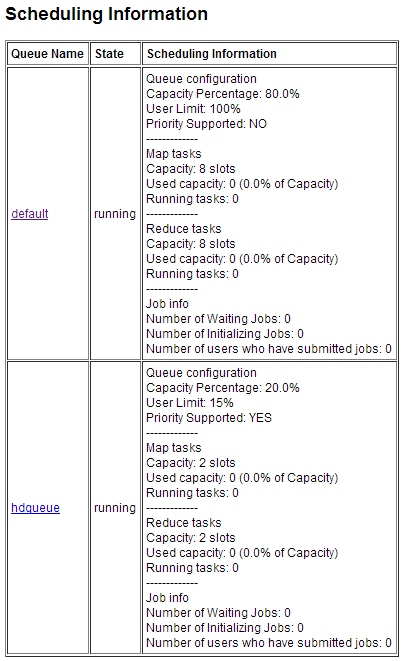
\includegraphics[width=.55\textwidth]{figs/5163os_04_17.png}
  \caption{Hadoop MapReduce job Scheduling information}\label{fig:mapred.scheduling}
\end{figure} 
Alternatively, we can use the command hadoop queue -list to get the same information. 

Get the schedule details of each queue by opening the URL, master:50030/scheduler, and we can get a web page similar to the following: 
\begin{figure}[ht]
  \centering
  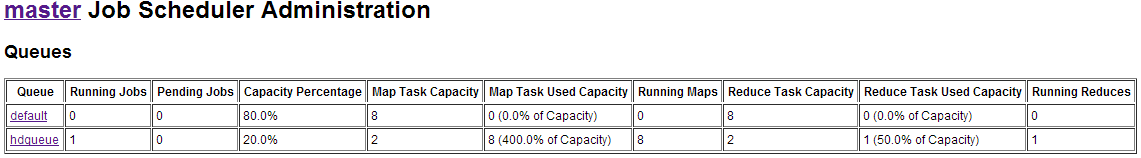
\includegraphics[width=.90\textwidth]{figs/5163os_04_18.png}
  \caption{Job Scheduler Queues}\label{fig:job.queues}
\end{figure} 
 Figure \ref{fig:job.queues} shows the status of each queue in the cluster including the numbers of running jobs, pending jobs, and so on. 

Test the queue configuration by submitting an example wordcount job to the queue hdqueue using the following command: 
\lstset{style=bashstyle}
\begin{lstlisting}[language=bash]
$ hadoop jar $HADOOP_HOME/hadoop-examples-1.1.2.jar wordcount -Dmapred.job.queue.name=hdqueue randtext wordcount.out
\end{lstlisting}

From the job information web UI, we can get the job scheduling information similar to the following: 
\lstset{style=bashstyle}
\begin{lstlisting}
Job Scheduling information: 8 running map tasks using 8 map slots. 0 additional slots reserved. 1 running reduce tasks using 1 reduce slots. 0 additional slots reserved.
\end{lstlisting}

\subsection*{How it works...}
CapacityScheduler is available as a JAR file under the \verb|$HADOOP_HOME/lib| directory. For example, in our Hadoop distribution, the JAR file is \verb|$HADOOP_HOME/lib/hadoop-capacity-scheduler-1.1.2.jar|.

Table \ref{tbl:queueconfig} shows the description of queue configuration properties: 
\begin{table}[ht]
  \scriptsize
  \centering
  \begin{tabular}{p{.45\textwidth}p{.45\textwidth}}
    \toprule 
    \textbf{Property} & \textbf{Description} \\ \midrule
    mapred.capacity-scheduler.queue.hdqueue.capacity & The percentage share of total number of slots for the hdqueue queue. \\
    mapred.capacity-scheduler.queue.default.capacity & The percentage share of total number of slots for default queue.\\
    mapred.capacity-scheduler.queue.hdqueue.minimum-user-limit-percent & The percentage of minimum resources allocated for each user in the queue hdqueue. \\
    mapred.capacity-scheduler.maximum-system-jobs & The maximum number of jobs that can be initialized concurrently by CapacityScheduler. \\
    mapred.capacity-scheduler.queue.hdqueue.maximum-initialized-active-tasks & The maximum number of concurrently initialized tasks across all jobs in the queue hdqueue. \\
    mapred.capacity-scheduler.queue.hdqueue.maximum-initialized-active-tasks-per-user & The maximum number of concurrently initialized tasks across all jobs in the queue hdqueue for each user. \\
    mapred.capacity-scheduler.queue.hdqueue.supports-priority & Whether to support job priority for job scheduling or not. \\ \bottomrule
  \end{tabular}
  \caption{Queue configuration related properties}\label{tbl:queueconfig}
\end{table}

\subsection*{There's more...}
Hadoop supports access control on the queue using queue ACLs. Queue ACLs control the authorization of MapReduce job submission to a queue. More information about queue ACLs can be found at \url{http://hadoop.apache.org/docs/r1.1.2/cluster_setup.html#Configuring+the+Hadoop+Daemons}.

\subsection*{See also}
\begin{itemize}
  \item The Managing MapReduce jobs recipe
  \item The Checking job history from the web UI recipe
  \item The Configuring Fair Scheduler recipe
  \item The Configuring job authentication with ACL recipe of Chapter \ref{chap:5}, Hardening a Hadoop Cluster
  \item Refer to \url{http://hadoop.apache.org/docs/r1.1.2/capacity_scheduler.html}
\end{itemize}

\section{Configuring Fair Scheduler}\index{FairScheduler}
Similar to CapacityScheduler, Fair Scheduler was designed to enforce fair shares of cluster resources in a multiuser environment. In this recipe, we will outline steps to configure Fair Scheduler for a Hadoop cluster.

\subsection*{Getting ready}
We assume that our Hadoop cluster has been configured properly and all the daemons are running without any problems.
Log in to the master node from the Hadoop administrator machine using the following command: \\
\verb|$ ssh hduser@master|

\subsection*{How to do it...}
Perform the following steps to configure Hadoop Fair Scheduler: 

Enable fair scheduling by changing the following property in the file \verb|$HADOOP_HOME/conf/mapred-site.xml|:
\begin{verbatim}[language=XML]
  <property>
    <name>mapred.jobtracker.taskScheduler</name>
    <value>org.apache.hadoop.mapred.FairScheduler</value>
  </property>
\end{verbatim}

Create the Fair Scheduler configuration file, \verb|$HADOOP_HOME/conf/fair-scheduler.xml|, with content similar to the following: 
\lstset{style=bashstyle}
\begin{lstlisting}[language=XML]
<?xml version="1.0"?> 
<allocations>
 <pool name="hduser">
    <minMaps>5</minMaps>
    <minReduces>5</minReduces>
    <maxMaps>90</maxMaps>
    <maxReduces>20</maxReduces>
    <weight>2.0</weight>
  </pool>
  <user name="hduser">
    <maxRunningJobs>1</maxRunningJobs>
  </user>
  <userMaxJobsDefault>3</userMaxJobsDefault>
</allocations>
\end{lstlisting}

Restart the MapReduce cluster with the following commands:
\lstset{style=bashstyle}
\begin{lstlisting}[language=bash]
$ stop-mapred.sh
$ start-mapred.sh
\end{lstlisting}

Verify the setting of Fair Scheduler by opening the URL \url{http://master:50030/scheduler}.

The web page will be similar to Figure \ref{fig:fairscheduler}.
\begin{figure}[ht]
  \centering
  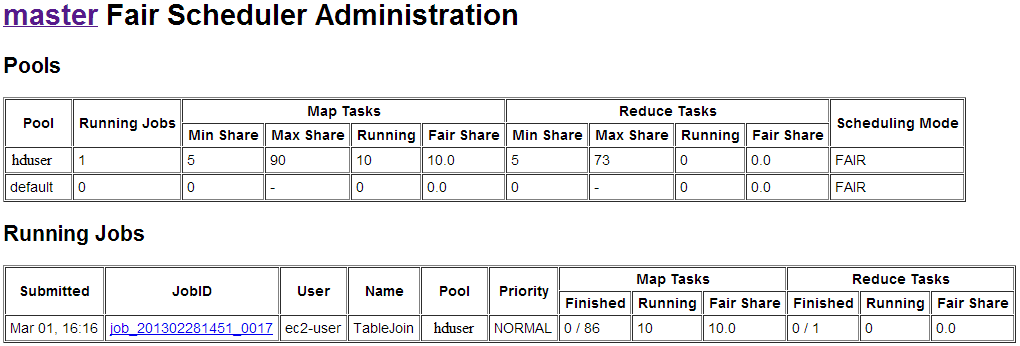
\includegraphics[width=.90\textwidth]{figs/5163os_04_16.png}
  \caption{Status of fair scheduler}\label{fig:fairscheduler}
\end{figure} 
\subsection*{How it works...}
The Hadoop Fair Scheduler schedules jobs in such a way that all jobs can get an equal share of computing resources. Jobs are organized with scheduling pools\index{scheduling pool}. A pool can be configured for each Hadoop user. If the pool for a user is not configured, the default pool will be used. A pool specifies the amount of resources a user can share on the cluster, for example the number of map slots, reduce slots, the total number of running jobs, and so on.

\emph{minMaps} and \emph{minReduces} are used to ensure the minimum share\index{minimum share} of computing slots on the cluster for a pool. The minimum share guarantee can be useful when the required number of computing slots is larger than the number of configured slots. In case if the minimum share of a pool is not met, JobTracker will kill tasks on other pools and assign the slots to the starving pool. In such cases, the JobTracker will restart the killed tasks on other nodes and thus, the job will take longer time to finish.

Besides computing slots\index{computing slots}, the Fair Scheduler can limit the number of concurrently running jobs and tasks on a pool. So, if a user submits more jobs than the configured limit, some jobs have to in-queue until other jobs finish. In such a case, higher priority jobs will be scheduled by the Fair Scheduler to run earlier than lower priority jobs. If all jobs in the waiting queue have the same priority, the Fair Scheduler can be configured to schedule these jobs with either Fair Scheduler or FIFO Scheduler\index{FIFO scheduler}.

Table \ref{tbl:fairscheduler} shows the properties supported by fair scheduler:
\begin{table}[ht]
  \centering
  \scriptsize
  \begin{tabular}{llp{9cm}}
    \toprule 
    \textbf{Property} & \textbf{Value} & \textbf{Description} \\ \midrule
    minMaps & Integer & Minimum map slots for a pool. \\
    maxMaps & Integer & Maximum map slots for a pool.\\
    minReduces & Integer & Minimum reduce slots for a pool.\\
    minReduces & Integer & Maximum reduce slots for a pool.\\
    schedulingMode & Fair/FIFO & Pool internal scheduling mode, fair or fifo. \\
    maxRunningJobs & Integer & Maximum number of concurrently running jobs for a pool. Default value is unlimited. \\
    weight & Float & Value to control non proportional share of cluster resource. The default value is 1.0. \\
    minSharePreemptionTimeout & Integer & Seconds to wait before killing other pool's tasks if a pool's share is under minimum share. \\
    maxRunningJobs & Integer & Maximum number of concurrent running jobs for a user. Default is unlimited.\\
    poolMaxJobsDefault & Integer & Default maximum number of concurrently running jobs for a pool.\\
    userMaxJobsDefault & Integer & Default maximum number of concurrently running jobs for a user. \\
    defaultMinSharePreemptionTimeout & Integer & Default seconds to wait before killing other pool's tasks when a pool's share is under minimum share. \\
    fairSharePreemptionTimeout & Integer & Pre-emption time when a job's resource is below half of the fair share.\\
    defaultPoolSchedulingMode & Fair/FIFO & Default in-pool scheduling mode. \\ \bottomrule
  \end{tabular}
  \caption{FairScheduler configuration properties}\label{tbl:fairscheduler}
\end{table}
\subsection*{See also}
\begin{itemize}
\item The Configuring CapacityScheduler recipe
\item Refer to \href{http://hadoop.apache.org/docs/r1.1.2/fair_scheduler.html}{the FairScheduler documentation}.
\end{itemize}

\section{Configuring Hadoop daemon logging}\index{daemon logging}
System logging plays an important role in dealing with performance and security problems. In addition, the logging information can be used analytically to tune the performance of a Hadoop cluster. In this recipe, we will show you how to configure Hadoop logging.

\subsection*{Getting ready}
We assume that our Hadoop cluster has been properly configured.

\subsection*{How to do it...}
Perform the following steps to configure Hadoop logging: 

Log in to the master node with the following command from the Hadoop administrator machine: \\ 
\verb|$ ssh hduser@master|

Check the current logging level of JobTracker with the following command:
\lstset{style=bashstyle}
\begin{lstlisting}
hadoop daemonlog -getlevel master:50030 org.apache.hadoop.mapred.JobTracker
Connecting to http://master:50030/logLevel?log=org.apache.hadoop.mapred.JobTracker
Submitted Log Name: org.apache.hadoop.mapred.JobTracker
Log Class: org.apache.commons.logging.impl.Log4JLogger
Effective level: INFO
\end{lstlisting}

Tell Hadoop to only log error events for JobTracker using the following command:
\lstset{style=bashstyle}
\begin{lstlisting}
$ hadoop daemonlog -setlevel master:50030 org.apache.hadoop.mapred.JobTracker ERROR
Connecting to http://master:50030/logLevel?log=org.apache.hadoop.mapred.JobTracker&level=ERROR
Submitted Log Name: org.apache.hadoop.mapred.JobTracker
Log Class: org.apache.commons.logging.impl.Log4JLogger
Submitted Level: ERROR
Setting Level to ERROR ...
Effective level: ERROR
\end{lstlisting}
Now, the logging status of the JobTracker daemon will be similar to the following:
\lstset{style=bashstyle}
\begin{lstlisting}
Connecting to http://master:50030/logLevel?log=org.apache.hadoop.mapred.JobTracker
Submitted Log Name: org.apache.hadoop.mapred.JobTracker
Log Class: org.apache.commons.logging.impl.Log4JLogger
Effective level: ERROR
\end{lstlisting}

Get the log levels for TaskTracker, NameNode, and DataNode with the following commands:
\lstset{style=bashstyle}
\begin{lstlisting}
hadoop daemonlog -getlevel master:50030 org.apache.hadoop.mapred.TaskTracker hadoop daemonlog -getlevel master:50070 org.apache.hadoop.dfs.NameNode
hadoop daemonlog -getlevel master:50070 org.apache.hadoop.dfs.DataNode
Connecting to http://master:50030/logLevel?log=org.apache.hadoop.mapred.TaskTracker
Submitted Log Name: org.apache.hadoop.mapred.TaskTracker
Log Class: org.apache.commons.logging.impl.Log4JLogger
Effective level: WARN

Connecting to http://master:50070/logLevel?log=org.apache.hadoop.dfs.NameNode
Submitted Log Name: org.apache.hadoop.dfs.NameNode
Log Class: org.apache.commons.logging.impl.Log4JLogger
Effective level: INFO

Connecting to http://master:50070/logLevel?log=org.apache.hadoop.dfs.DataNode
Submitted Log Name: org.apache.hadoop.dfs.DataNode
Log Class: org.apache.commons.logging.impl.Log4JLogger
Effective level: INFO
\end{lstlisting}

\subsection*{How it works...}
By default, Hadoop sends log messages to Log4j, which is configured in the file \verb|$HADOOP_HOME/conf/log4j.properties|. This file defines both what to log and where to log. For applications, the default root logger is INFO,console , which logs all messages at level INFO and above the console's stderr. Log files are named \verb|$HADOOP_LOG_DIR/hadoop-$HADOOP_IDENT_STRING-<hostname>.log|.

Hadoop supports a number of log levels for different purposes. The log level should be tuned based on the purpose of logging. For example, if we are debugging a daemon, we can set its logging level to be DEBUG rather than something else. Using a verbose log level can give us more information, while on the other hand will incur overhead to the cluster.

Table \ref{tbl:log4j} shows all the logging levels provided by Log4j:
\begin{table}
  \begin{tabular}{ll}
    \toprule 
    \textbf{Log level} & \textbf{Description} \\ \midrule
    ALL & The lowest logging level, all loggings will be turned on. \\
    DEBUG & Logging events useful for debugging applications.\\
    ERROR & Logging error events, but application can continue to run. \\
    FATAL & Logging very severe error events that will abort applications. \\
    INFO & Logging informational messages that indicate the progress of applications. \\
    OFF & Logging will be turned off. \\
    TRACE & Logging more finger-grained events for application debugging. \\
    \verb|TRACE_INT| & Logging in TRACE level on integer values. \\
    WARN & Logging potentially harmful events. \\ \bottomrule
  \end{tabular}
  \caption{Log4j logging levels}\label{tbl:log4j}
\end{table}

We can get the usage of daemonlog with the following command:
\lstset{style=bashstyle}
\begin{lstlisting}
$ hadoop daemonlog
USAGES:
java org.apache.hadoop.log.LogLevel -getlevel <host:port> <name>
java org.apache.hadoop.log.LogLevel -setlevel <host:port> <name> <level>
\end{lstlisting}

\subsection*{There's more...}
Other than configuring Hadoop logging on the fly from command line, we can configure it using configuration files. The most important file that we need to configure is \verb|$HADOOP/conf/hadoop-env.sh|.

Sometimes, audit logging\index{audit logging} is desirable for corporate auditing purposes. Hadoop provides audit logging through Log4j\index{log4j} using the INFO logging level. We will show you how to configure Hadoop audit logging in the next recipe.

The cluster needs to be restarted for the configuration to take effect.

\subsubsection*{Configuring Hadoop logging with hadoop-env.sh}
Open the file \verb|$HADOOP_HOME/conf/hadoop-env.sh| with a text editor and change the following line: \\
\verb|# export HADOOP_LOG_DIR=${HADOOP_HOME}/logs|

We change the preceding command to the following: \\
\verb|export HADOOP_LOG_DIR=${HADOOP_HOME}/logs|

Configure the logging directory to \verb|/var/log/hadoop| by changing the following line: \\
\verb|export HADOOP_LOG_DIR=/var/log/hadoop|

Additionally, Table \ref{tbl:loggingenv} shows other environment variables we can configure for Hadoop logging:
\begin{table}\scriptsize\centering
  \begin{tabular}{ll}
    \toprule 
    Variable name & Description \\ midrule
    \verb|HADOOP_LOG_DIR| & Directory for log files. \\ 
    \verb|HADOOP_PID_DIR| & Directory to store the PID for the servers. \\
    \verb|HADOOP_ROOT_LOGGER| & Logging configuration for hadoop.root.logger. Default value: "INFO,console". \\
    \verb|HADOOP_SECURITY_LOGGER| & Logging configuration for hadoop.security.logger. Default value: "INFO,NullAppender".\\
    \verb|HDFS_AUDIT_LOGGER| & Logging configuration for hdfs.audit.logger. Default value: "INFO,NullAppender".\\ \bottomrule 
  \end{tabular}
  \caption{Environment variables related to logging}\label{tbl:loggingenv}
\end{table}

\section{Configuring Hadoop security logging}\index{security logging}
Security logging can help Hadoop cluster administrators to identify security problems. It is enabled by default.

The security logging configuration is located in the file \verb|$HADOOP_HOME/conf/log4j.properties|. By default the security logging information is appended to the same file as NameNode logging. We can check the security logs with the following command:
\lstset{style=bashstyle}
\begin{lstlisting}
grep security $HADOOP_HOME/logs/hadoop-hduser-namenode-master.log
2013-02-28 13:36:01,008 ERROR org.apache.hadoop.security.UserGroupInformation: PriviledgedActionException as:hduser cause:org.apache.hadoop.hdfs.server.namenode.SafeModeException: Cannot create file/user/hduser/test. Name node is in safe mode.
\end{lstlisting}

The error message tells that the NameNode is in safe mode, so the file \verb|/user/hduser/test| cannot be created. Similar information can give us a very useful hint to figure out operation errors.

\subsubsection*{Hadoop logging file naming conventions}
Hadoop logs files are kept under the directory \verb|$HADOOP_HOME/logs|. 

The folder contains one .log file and one .out file for each Hadoop daemon, for example, NameNode, SecondaryNameNode, and JobTracker on the master node and TaskTracker and DataNode on a slave node. The .out file is used when a daemon is being started. Its content will be emptied after the daemon has started successfully. The .log files contain all the log messages for a daemon, including startup logging messages.

On the master node, the logs directory contains a history folder that contains logs of the MapReduce job history. Similarly, on a slave node, the logs directory contains a userlogs directory, which maintains the history information of the tasks that ran on the node.

In Hadoop, the names of logging files are using the following format: \\
\verb|$ hadoop-<username>-<daemonname>-<hostname>.log |
\subsection*{See also}
\begin{itemize}
  \item The Configuring Hadoop audit logging recipe
  \item Refer to \url{http://wiki.apache.org/hadoop/HowToConfigure}
\end{itemize}
\section{Configuring Hadoop audit logging}
Audit logging might be required for data processing systems such as Hadoop. In Hadoop, audit logging has been implemented using the Log4j Java logging library at the INFO logging level. By default, Hadoop audit logging is disabled. This recipe will guide you through the steps to configure Hadoop audit logging.

\subsection*{Getting ready}
We assume that our Hadoop cluster has been configured properly.
Log in to the master node from the administrator machine using the following command:\\ 
\verb|$ ssh hduser@master|

\subsection*{How to do it...}
Perform the following steps to configure Hadoop audit logging: 

Enable audit logging by changing the following line in the \verb|$HADOOP_HOME/conf/log4j.properties| file from: 
\lstset{style=bashstyle}
\begin{lstlisting}
log4j.logger.org.apache.hadoop.hdfs.server.namenode.FSNamesystem.audit=WARN
\end{lstlisting}

to the following:
\lstset{style=bashstyle}
\begin{lstlisting}
log4j.logger.org.apache.hadoop.hdfs.server.namenode.FSNamesystem.audit=INFO
\end{lstlisting}

Try making a directory on HDFS with the following command: \\
\verb|$ hadoop fs -mkdir audittest|

Check the audit log messages in the NameNode log file with the following command:
\lstset{style=bashstyle}
\begin{lstlisting}
$ grep org.apache.hadoop.hdfs.server.namenode.FSNamesystem.audit $HADOOP_HOME/logs/hadoop-hduser-namenode-master.log
2013-02-28 13:38:04,235 INFO org.apache.hadoop.hdfs.server.namenode.FSNamesystem.audit: ugi=hduser    ip=/10.0.0.1  cmd=mkdirs   src=/user/hduser/audittest  dst=null        perm=hduser:supergroup:rwxr-xr-x
\end{lstlisting}
The Hadoop NameNode is responsible for managing audit logging messages, which are forwarded to the NameNode logging facility. So what we have seen so far is that the audit logging message has been mixed with the normal logging message.

We can separate the audit logging messages from the NameNode logging messages by configuring the file \verb|$HADOOP_HOME/conf/log4j.properties| with the following content: 
\lstset{style=bashstyle}
\begin{lstlisting}
# Log at INFO level, SYSLOG appenders
log4j.logger.org.apache.hadoop.hdfs.server.namenode.FSNamesystem.audit=INFO

# Disable forwarding the audit logging message to the NameNode logger.
log4j.additivity.org.apache.hadoop.hdfs.server.namenode.FSNamesystem.audit=false

################################
# Configure logging appender
################################
#
# Daily Rolling File Appender (DRFA)
log4j.appender.DRFAAUDIT=org.apache.log4j.DailyRollingFileAppender
log4j.appender.DRFAAUDIT.File=$HADOOP_HOME/logs/audit.log
log4j.appender.DRFAAUDIT.DatePattern=.yyyy-MM-dd
log4j.appender.DRFAAUDIT.layout=org.apache.log4j.PatternLayout
log4j.appender.DRFAAUDIT.layout.ConversionPattern=%d{ISO8601} %p %c: %m%n
\end{lstlisting}

\subsection*{How it works...}
Hadoop logs auditing messages of operations, such as creating, changing, or deleting files into a configured log file. By default, audit logging is set to \emph{WARN}, which disables audit logging. To enable it, the logging level need be changed to \emph{INFO}.

When a Hadoop cluster has many jobs to run, the log file can become large very quickly. Log file rotation is a function that periodically rotates a log file to a different name, for example, by appending the date to the filename, so that the original log file name can be used as an empty file.
\subsection*{See also}
\begin{itemize}
  \item The Configuring Hadoop daemon logging recipe
\end{itemize}

\section{Upgrading Hadoop}\index{upgrading hadoop}
A Hadoop cluster needs to be upgraded when new versions with bug fixes or new features are released. In this recipe, we will outline steps to upgrade a Hadoop cluster to a newer version.

\subsection*{Getting ready}
Download the desired Hadoop release from an Apache mirror site: \url{http://www.apache.org/dyn/closer.cgi/hadoop/common/}. In this book, we assume to upgrade Hadoop from version \emph{1.1.2} to version \emph{1.2.0}, which is still in the beta state when writing this book.

We assume that there are no running or pending MapReduce jobs in the cluster.

In the processing of upgrading a Hadoop cluster, we want to minimize the damage to the data stored on HDFS, and this procedure is the cause of most of the upgrade problems. The data damages can be caused by either human operation or software and hardware failures. So, a backup of the data might be necessary. But the sheer size of the data on HDFS can be a headache for most of the upgrade experience.

A more practical way is to only back up the HDFS filesystem metadata on the master node, while leaving the data blocks intact. If some data blocks are lost after upgrade, Hadoop can automatically recover it from other backup replications.

Log in to the master node from the administrator machine with the following command: \\
\verb|$ ssh hduser@master|

\subsection*{How to do it...}
Perform the following steps to upgrade a Hadoop cluster: 

Stop the cluster with the following command: \\
\verb|$ stop-all.sh|

Back up block locations of the data on HDFS with the fsck command:
\lstset{style=bashstyle}
\begin{lstlisting}[language=bash]
$ hadoop fsck / -files -blocks -locations > dfs.block.locations.fsck.backup
\end{lstlisting}

The resulting file, \verb|dfs.block.locations.fsck.backup|, will contain the locations of each data block on the HDFS filesystem.

Save the list of all files on the HDFS filesystem with the following command: \\
\verb|$ hadoop dfs -lsr / > dfs.namespace.lsr.backup|

Save the description of each DataNode in the HDFS cluster with the following command: \\ 
\verb|$ hadoop dfsadmin -report > dfs.datanodes.report.backup| 

Copy the checkpoint files to a backup directory with the following commands:
\lstset{style=bashstyle}
\begin{lstlisting}[language=bash]
$ sudo cp dfs.name.dir/edits /backup
$ sudo cp dfs.name.dir/image/fsimage /backup
\end{lstlisting}

Verify that no DataNode daemon is running with the following command:
\lstset{style=bashstyle}
\begin{lstlisting}[language=bash]
for node in `cat $HADOOP_HOME/conf/slaves`
  do
  echo 'Checking node ' $node
  ssh $node -C "jps"
done
\end{lstlisting}
If any DataNode process is still running, kill the process with the following command:
\lstset{style=bashstyle}
\begin{lstlisting}[language=bash]
$ ssh $node -C "jps | grep 'DataNode' | cut -d'\t' -f 1 | xargs kill -9 "
\end{lstlisting}

A still running DataNode can fail an update if it is not killed because the old version DataNode might register with the newer version NameNode, causing compatibility problems.

Decompress the Hadoop archive file with the following commands:
\lstset{style=bashstyle}
\begin{lstlisting}[language=bash]
$ sudo mv hadoop-1.2.0.tar.gz /usr/local/
$ sudo tar xvf hadoop-1.2.0.tar.gz
\end{lstlisting}

Copy the configuration files from the old configuration directory to the new one using the following command: \\
\verb|$ sudo cp $HADOOP_HOME/conf/* /usr/local/hadoop-1.2.0/conf/*| \\ 

You can make changes to the configuration files if necessary.

Update the Hadoop symbolic link to the Hadoop version with the following command:
\lstset{style=bashstyle}
\begin{lstlisting}[language=bash]
$ sudo rm -rf /usr/local/hadoop
$ sudo ln -s /usr/local/hadoop-1.2.0 /usr/local/hadoop
\end{lstlisting}

Upgrade in the slave nodes with the following commands:
\lstset{style=bashstyle}
\begin{lstlisting}[language=bash]
for host in `cat $HADOOP_HOME/conf/slaves`
  do
  echo 'Configuring hadoop on slave node ' $host
  sudo scp -r /usr/local/hadoop-1.2.0 hduser@$host:/usr/local/
  echo 'Making symbolic link for Hadoop home directory on host ' $host
  sudo ssh hduser@$host -C "ln -s /usr/local/hadoop-1.2.0 /usr/local/hadoop"
done
\end{lstlisting}

Upgrade the NameNode with the following command: \\
\verb|$ hadoop namenode -upgrade| 

This command will convert the checkpoint to the new version format. We need to wait to let it finish.

Start the HDFS cluster using the following commands: \\
\verb|$ start-dfs.sh| 

Get the list of all files on HDFS and compare its difference with the backed up one using the following commands:
\lstset{style=bashstyle}
\begin{lstlisting}[language=bash]
$ hadoop dfs -lsr / > dfs.namespace.lsr.new
$ diff dfs.namespace.lsr.new dfs.namespace.lsr.backup
\end{lstlisting}

The two files should have the same content if there is no error in the upgrade. 

Get a new report of each DataNode in the cluster and compare the file with the backed up one using the following command:
\lstset{style=bashstyle}
\begin{lstlisting}[language=bash]
$ hadoop dfsadmin -report > dfs.datanodes.report.new
$ diff dfs.datanodes.report.1.log dfs.datanodes.report.backup
\end{lstlisting}

The two files should have the same content if there is no error.

Get the locations of all data blocks and compare the output with the previous backup using the following commands:
\lstset{style=bashstyle}
\begin{lstlisting}[language=bash]
$ hadoop fsck / -files -blocks -locations > dfs.block.locations.fsck.new
$ diff dfs.locations.fsck.backup dfs.locations.fsck.new
\end{lstlisting}

The result of this command should tell us that the data block locations should be the same. 

Start the MapReduce cluster using the following command: \\ 
\verb|$ start-mapred.sh| 

Now, we can check the status of the cluster either by running a sample MapReduce job such as teragen and terasort, or by using the web user interface.

\subsection*{How it works...}
We can use the following command to get the usage of HDFS upgrade commands:
\lstset{style=bashstyle}
\begin{lstlisting}
$ hadoop dfsadmin

Usage: java DFSAdmin
           [-report]
           [-safemode enter | leave | get | wait]
           [-saveNamespace]
           [-refreshNodes]
           [-finalizeUpgrade]
           [-upgradeProgress status | details | force]
           [-metasave filename]
           [-refreshServiceAcl]
           [-refreshUserToGroupsMappings]
           [-refreshSuperUserGroupsConfiguration]
           [-setQuota <quota> <dirname>...<dirname>]
           [-clrQuota <dirname>...<dirname>]
           [-setSpaceQuota <quota> <dirname>...<dirname>]
           [-clrSpaceQuota <dirname>...<dirname>]
           [-setBalancerBandwidth <bandwidth in bytes per second>]
           [-help [cmd]]
\end{lstlisting}

Table \ref{tbl:dfsadmin} shows the meanings of the command options:
\begin{table}
  \centering
  \small
  \begin{tabular}{lp{.75\textwidth}}
    \toprule 
    \textbf{Option} & \textbf{Description} \\ \midrule 
    -report & Reports filesystem information and statistics. \\ 
    -saveNamespace & Save a snapshot of the filesystem metadata into configured directories. \\
    -finalizeUpgrade & Finalize the upgrade of HDFS; this command will cause the DataNode to delete the previous version working directories. \\
    -metasave & Saves the metadata of the HDFS cluster. \\ \bottomrule 
  \end{tabular}
  \caption{DFSAdmin command options}\label{tbl:dfsadmin}
\end{table}

\subsection*{See also}
\begin{itemize}
  \item The Configuring Hadoop in pseudo-distributed mode recipe of Chapter \ref{chap:3}, Configuring a Hadoop Cluster
  \item The Configuring Hadoop in fully-distributed mode recipe of Chapter \ref{chap:3}, Configuring a Hadoop Cluster
  \item The Validating Hadoop installation recipe of Chapter \ref{chap:3}, Configuring a Hadoop Cluster
\end{itemize}
